%%%%%%%%%%%%%%%%%%%%%%%%%%%%% Define Article %%%%%%%%%%%%%%%%%%%%%%%%%%%%%%%%%%
\documentclass[a4paper]{article}
%%%%%%%%%%%%%%%%%%%%%%%%%%%%%%%%%%%%%%%%%%%%%%%%%%%%%%%%%%%%%%%%%%%%%%%%%%%%%%%

%%%%%%%%%%%%%%%%%%%%%%%%%%%%% Using Packages %%%%%%%%%%%%%%%%%%%%%%%%%%%%%%%%%%
\usepackage{geometry}
\usepackage{graphicx}
\usepackage{amssymb}
\usepackage{amsmath}
\usepackage{amsthm}
\usepackage{booktabs}
\usepackage{lipsum}
\usepackage{graphicx}
\usepackage{color}
\usepackage{nth}
\usepackage{bm}
\usepackage{caption}
\usepackage{subcaption}
\usepackage{url}
\usepackage{hyperref}
\usepackage{array}
\usepackage{multirow}
\usepackage{parskip}
\usepackage{xcolor}
%%%%%%%%%%%%%%%%%%%%%%%%%% Page Setting %%%%%%%%%%%%%%%%%%%%%%%%%%%%%%%%%%%%%%%
\geometry{a4paper}

% sans-serif font
\renewcommand{\familydefault}{\sfdefault}

%%%%%%%%%%%%%%%%%%%%%%%%%% Define some useful colors %%%%%%%%%%%%%%%%%%%%%%%%%%
\definecolor{ocre}{RGB}{243,102,25}
\definecolor{mygray}{RGB}{243,243,244}
\definecolor{deepGreen}{RGB}{26,111,0}
\definecolor{shallowGreen}{RGB}{235,255,255}
\definecolor{deepBlue}{RGB}{61,124,222}
\definecolor{shallowBlue}{RGB}{235,249,255}

\definecolor{darkGreen}{RGB}{47,125,73}
\definecolor{darkRed}{RGB}{196, 49, 25}

\newcommand{\posHi}[1]{\textcolor{darkGreen}{\textbf{#1}}}
\newcommand{\negHi}[1]{\textcolor{darkRed}{\textbf{#1}}}
%%%%%%%%%%%%%%%%%%%%%%%%%%%%%%%%%%%%%%%%%%%%%%%%%%%%%%%%%%%%%%%%%%%%%%%%%%%%%%%

%%%%%%%%%%%%%%%%%%%%%%%%%% Macros %%%%%%%%%%%%%%%%%%%%%%%%%%%%%%%%%%%%%%%%%%%%%
\DeclareMathOperator{\Lagr}{\mathcal{L}}
%%%%%%%%%%%%%%%%%%%%%%%%%%%%%%%%%%%%%%%%%%%%%%%%%%%%%%%%%%%%%%%%%%%%%%%%%%%%%%%


\begin{document}
% custom title page
\begin{titlepage}
  \begin{center}

    \vspace*{1cm}

    \textbf{\LARGE
    % Training and Deploying Computer Vision Models for Indoor Localisation
    % Exploring Deep Learning for Indoor Localisation: A Study on Room-Level Accuracy
    Navigating Indoors with Computer Vision: Exploring Deep Learning Approaches
    for Room-Level Indoor Localisation
    % Deep Learning for Accurate Room-Level Indoor Localisation: Feasibility and Evaluation
    % Enhancing Indoor Spatial Awareness: Deep Learning Approaches for Room-Level
    % Indoor Localisation
    }

    \vspace{1.5cm}

    % author
    \begin{minipage}[t]{5cm}
      \centering
      \textbf{Mika Senghaas} (Author) \\
      IT University of Copenhagen \\
      \textit{jsen@itu.dk}
    \end{minipage}
    \hspace{1cm}
    \begin{minipage}[t]{5cm}
      \centering
      \textbf{Stella Grasshof} (Supervisor) \\
      IT University of Copenhagen \\
      \textit{stgr@itu.dk}
    \end{minipage}

    \vfill

    % degree
    A Thesis presented for the Degree of \\
    \textbf{Bachelor of Science in Data Science}

    \vspace{0.8cm}

    
\includegraphics[width=0.4\textwidth]{figures/itu.jpg}

    \vspace{0.8cm}

    \textbf{IT University of Copenhagen}\\
    Computer Science Department\\
    \vspace{.5cm}
    May, 15th 2023

  \end{center}
\end{titlepage}

\newpage

% table of contents, list of tables, list of figures
\tableofcontents
% \listoftables
% \listoffigures
\newpage

\begin{abstract} % (fold)

In an increasingly urbanised and digitalised world, indoor localisation is
becoming a necessity for a wide variety of applications, ranging from personal
navigation to augmented reality. However, despite extensive research efforts,
indoor localisation remains a challenging task and no single solution is widely
adopted. Motivated by the success of deep learning in numerous computer vision
tasks, this study explores the feasibility of deep learning for accurate
room-level localisation in indoor spaces. Various neural network architectures
are trained and evaluated on a novel video dataset tailored for indoor
localisation. The findings reveal that deep learning approaches can provide
reasonable localisation results, even when trained on a small dataset. The
approach is currently limited in its ability to distinguish between visually
similar and adjacent areas, as well as biases within the training data. Despite
these shortcomings, the results are encouraging and inspire optimism about the
method's practical viability.

\end{abstract}

\section{Introduction}
\label{sec:introduction}

% outdoor localisation as solved problem 
With the introduction of the satellite-based Global Positioning System
(GPS), localisation in outdoor spaces has become more efficient and accurate
than ever before. Gradual commercialisation led to the technology rapidly
transforming industries and personal navigation. Today, outdoor localisation is
widely considered a \textit{solved problem}.

% gps struggles in indoor spaces
The same cannot be said for indoor localisation. Because the transmitted radio
signals sent out by the satellites in GPS systems are not strong enough to
penetrate through walls and struggle with reflections from large buildings, the
technology yields inaccurate results at best, and often becomes dysfunctional in
indoor spaces~\cite{survey1, survey2}.

% indoor localisation techniques (broad overview)
With the ongoing urbanisation and the emergence of autonomous robots and
vehicles, the need for indoor localisation technologies is growing. Over the
past decade, a wide variety of solutions have been proposed.
Infrastructure-based systems use radio signals transmitted by beacons, like
Bluetooth~\cite{bluetooth1, bluetooth2}, Ultra-Wideband (UWB)~\cite{uwb1, uwb2}
or Wi-Fi~\cite{survey1, survey2, wireless-positioning}, to localise an agent in
a known environment. Infrastructure-less systems, like simultaneous localisation
and mapping (SLAM) algorithms, rely solely on sensors, like
cameras~\cite{mono-slam, ptam, orb-slam} or distance-measuring
lasers~\cite{lidar-slam} to localise an agent in an unknown environment.

% short-comings of existing approaches
While these approaches have produced remarkable results, localising agent's with
centimetre accuracy, they are limited for various reasons: Infrastructure-based
systems require initial setup and maintenance of the installed hardware, which
makes them costly, time-intensive and difficult to implement in large
environments. Current infrastructure-less systems, on the other hand, require
complex hand-designed algorithms for processing the sensory information and need
to be fine-tuned by experts for each indoor space, to achieve outstanding
results. Much of the complexity of existing solutions is grounded in the
assumption that all applications require centimetre accuracy. However, not all
use-cases require such precision. For example, in a museum or shopping mall, it
might be sufficient to know in which area a visitor is. In these cases, the
constraint of centimetre accuracy can be relaxed, in favour of a simpler and
more versatile solution.

% success of deep learning in computer vision
Deep learning, which is part of a broader family of machine learning methods,
has recently gained a lot of attention in the field of computer vision and
proven to be a powerful tool for solving a wide variety of tasks. Common
computer vision tasks are image and video classification, where the goal is to
predict a label from a set of pre-defined labels for a given image or video. 

Given this, it is natural to ask (a) whether indoor localisation can be phrased
as a coarse-grained classification task, where labels correspond to areas in an
indoor space, and (b) whether deep learning techniques can be used to produce
accurate localisation results in this setting. Therefore, this study
investigates the applicability of modern deep learning techniques to indoor
localisation. The main contributions can be summarised as: 

\begin{enumerate} 

  \item A novel single-frame and video classification dataset tailored for
    indoor localisation.

  \item A rigorous evaluation of several modern deep learning architectures for
    the task of indoor localisation, when viewed as a classification task.

  \item A discussion of the results and an outlook on the applicability of a
    pure deep learning pipeline for indoor localisation.

\end{enumerate}


\section{Background} % (fold)
\label{sec:background}

Phrasing the problem of indoor localisation as a classification problem and
solving it with a pure deep learning approach requires a brief introduction to
some of the fundamentals that underlie this project's methods. This section,
therefore, introduces the fundamental concepts of deep learning relevant to this
study.

\subsection{Fundamentals of Machine and Deep Learning}

Machine learning is a subfield of artificial intelligence (AI) that describes a
series of techniques and algorithms that allow computers to learn from data
without being explicitly programmed. One example of a machine learning task is
classification, which aims to assign a discrete label $\hat{y} \in \{y_1,
\ldots, y_n\}$ to an input $x$. The mapping from the input $x$ to the label
$\hat{y}$ is called a classifier, and often denoted as $\hat{f}(x) = \hat{y}$.
Typically such a classifier is trained on a large set of labelled data, called
the training set, which consists of true instances $x_i$ and their labels $y_i$.
Using numeric optimisation algorithms, like gradient-descent, the classifier
iteratively improves its approximation $\hat{f}$ of the true mapping $f(x) = y$
by minimising a loss function $\mathcal{L}(\hat{f}(x), y)$ that quantifies the
error of the machine learning model.

Deep learning is a subfield of machine learning, and describes a specific class
of machine learning algorithms that are based on the theory of artificial neural
networks (ANNs). ANNs are inspired by and loosely related to the structure and
functioning of the neurons in the human brain. They are structured in a series
of fully-connected layers, where each layer consists of nodes.
Figure~\ref{fig:ann} shows an ANN with an input layer with three nodes, three
hidden layers with seven nodes each and an output layer with three nodes.
Information flows from the input layer through the hidden layers to the output
layer. The information flow happens through sequential linear transformations of
the input data, which are performed by the nodes in the network. Specifically,
each node's output is a linear transformation of the outputs of all nodes in the
previous layer, 

\begin{equation}
  z_{i} = \sum_{j=1}^{n} w_{ij} x_j + b_i
  \label{eq:perceptron}
\end{equation}

where $x_j$ is the output of the $j$-th node in the previous layer, $w_{ij}$ is
the weight of the connection between the $j$-th node in the previous layer and
the $i$-th node in the current layer, $b_i$ is the bias of the $i$-th node in
the current layer, and $z_i$ is the output of the node.

Before the output $z_i$ is passed to the next layer, it is transformed by a
differentiable, non-linear activation function $\sigma$ to produce an activation
$a_i = \sigma(z_i)$. Once all activations in the $j$-th layer are computed, the
next layer's activations can be computed in the same way. This process, referred
to as forward propagation, is iteratively repeated until the activations in the
output layer are computed, which are the final outputs of the network.

Critically, the linear transformations performed by each node are parametrised
by weights, which are optimised during training. This allows ANNs to learn
complex non-linear mappings given enough samples of the input-output
relationship without explicitly programming the mapping. The generality and
scalability of the method have proven ANNs to be a powerful tool for modelling
complex data relationships in a wide variety of domains.

\begin{figure}
  \begin{center}
    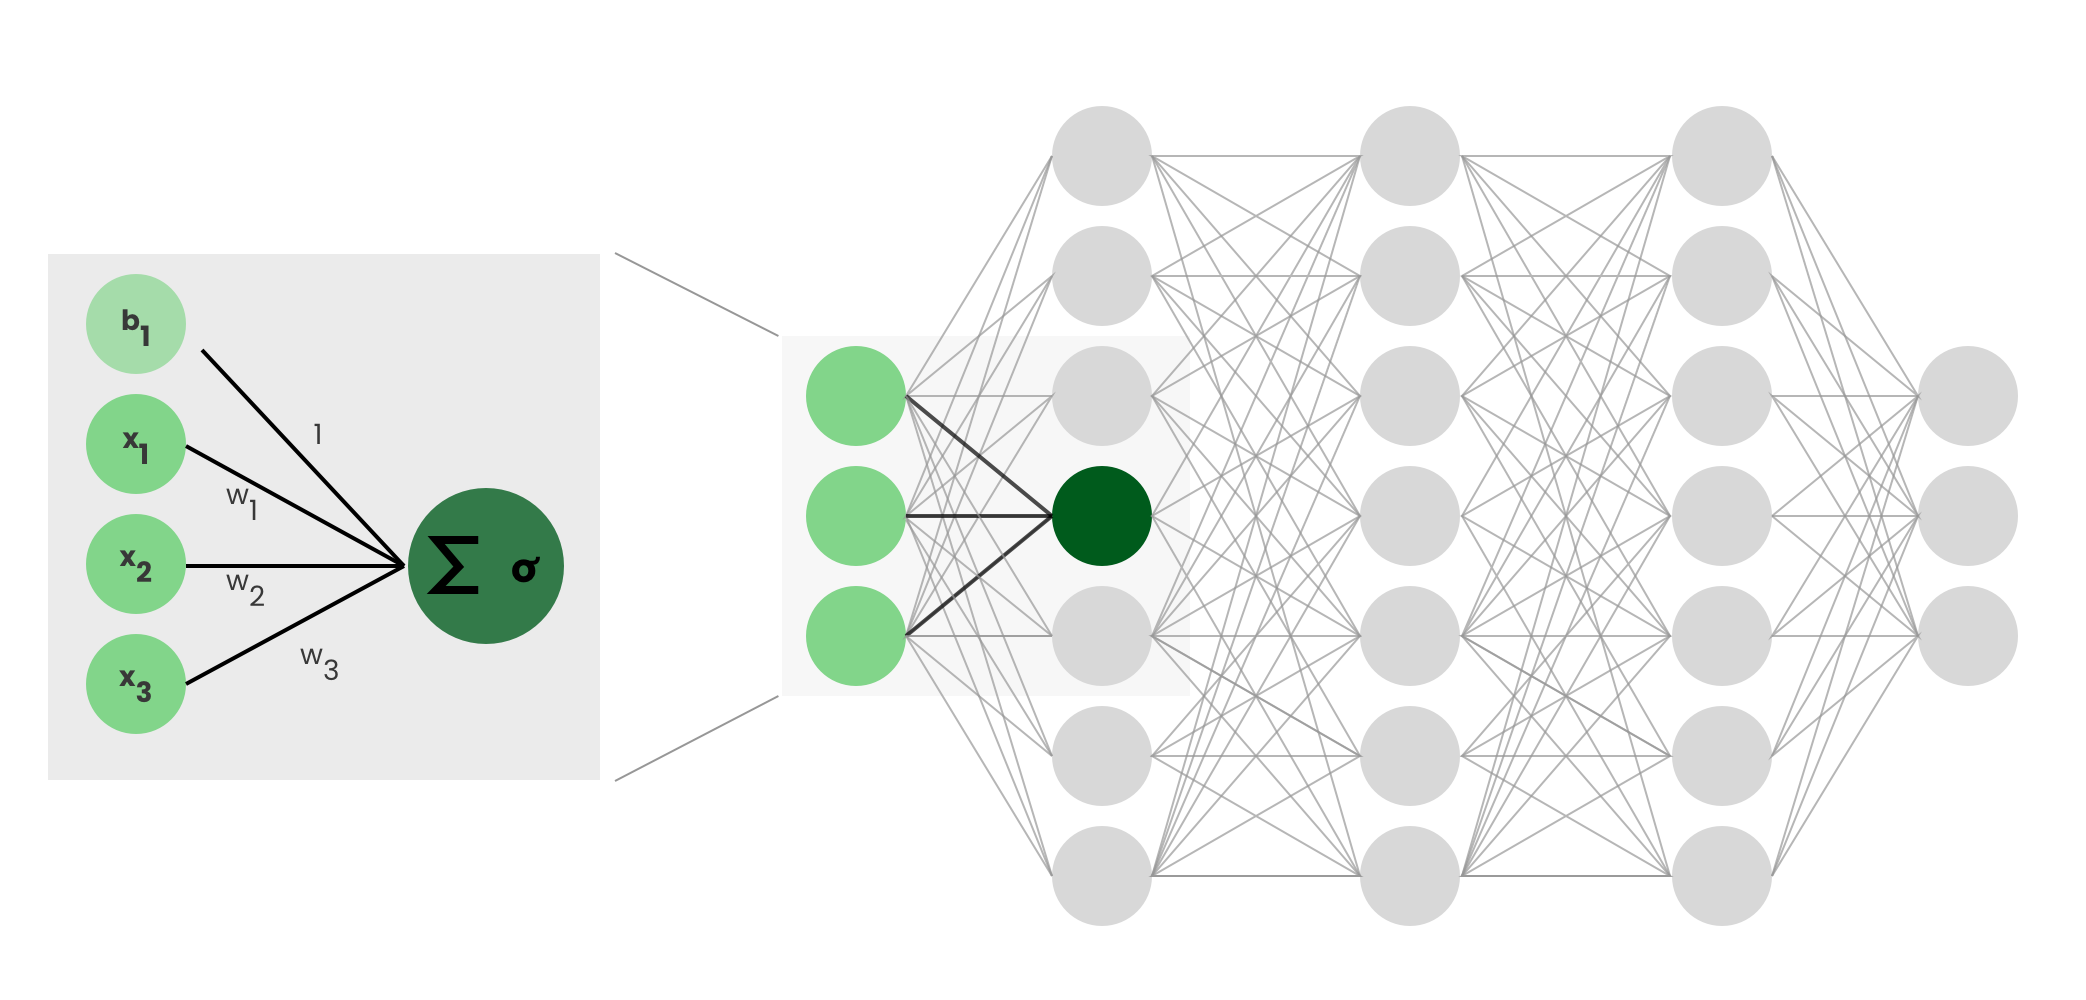
\includegraphics[width=\textwidth]{./figures/ann.png}
  \end{center}

  \caption{\textbf{Artificial Neural Network.} A schematic of the fundamental
    building blocks of an artificial neural network (ANN). The right figure
    shows the macro structure of an exemplary ANN with an input layer, three
    hidden layers, and an output layer. The left figure shows the micro
    structure of a single node in the network. The node performs a linear
    transformation of the inputs $x_i$ and the weights $w_i$ and adds a bias
    $b_i$. The output of the node is the result of a non-linear activation
    function $\sigma$ applied to the linear transformation.}
  \label{fig:ann}
\end{figure}

\subsection{Image Classification}
\label{sub:image-classification}

Image classification is one of the most fundamental and widely studied tasks in
computer vision and describes the process of assigning a label $y \in \{y_1,
\ldots, y_n\}$ to an image $x$. Extracting information from images to assign a
label is not straight-forward, because of the high-dimensional and unstructured
nature of images. These characteristics make it challenging for traditional
heuristic-based algorithms to extract meaningful information, which has long
limited the capabilities of computer vision systems. However, with the advent of
deep learning and the introduction of a special type of neural network, called
convolutional neural network (CNN), this has changed.

\begin{figure}
  \begin{center}
    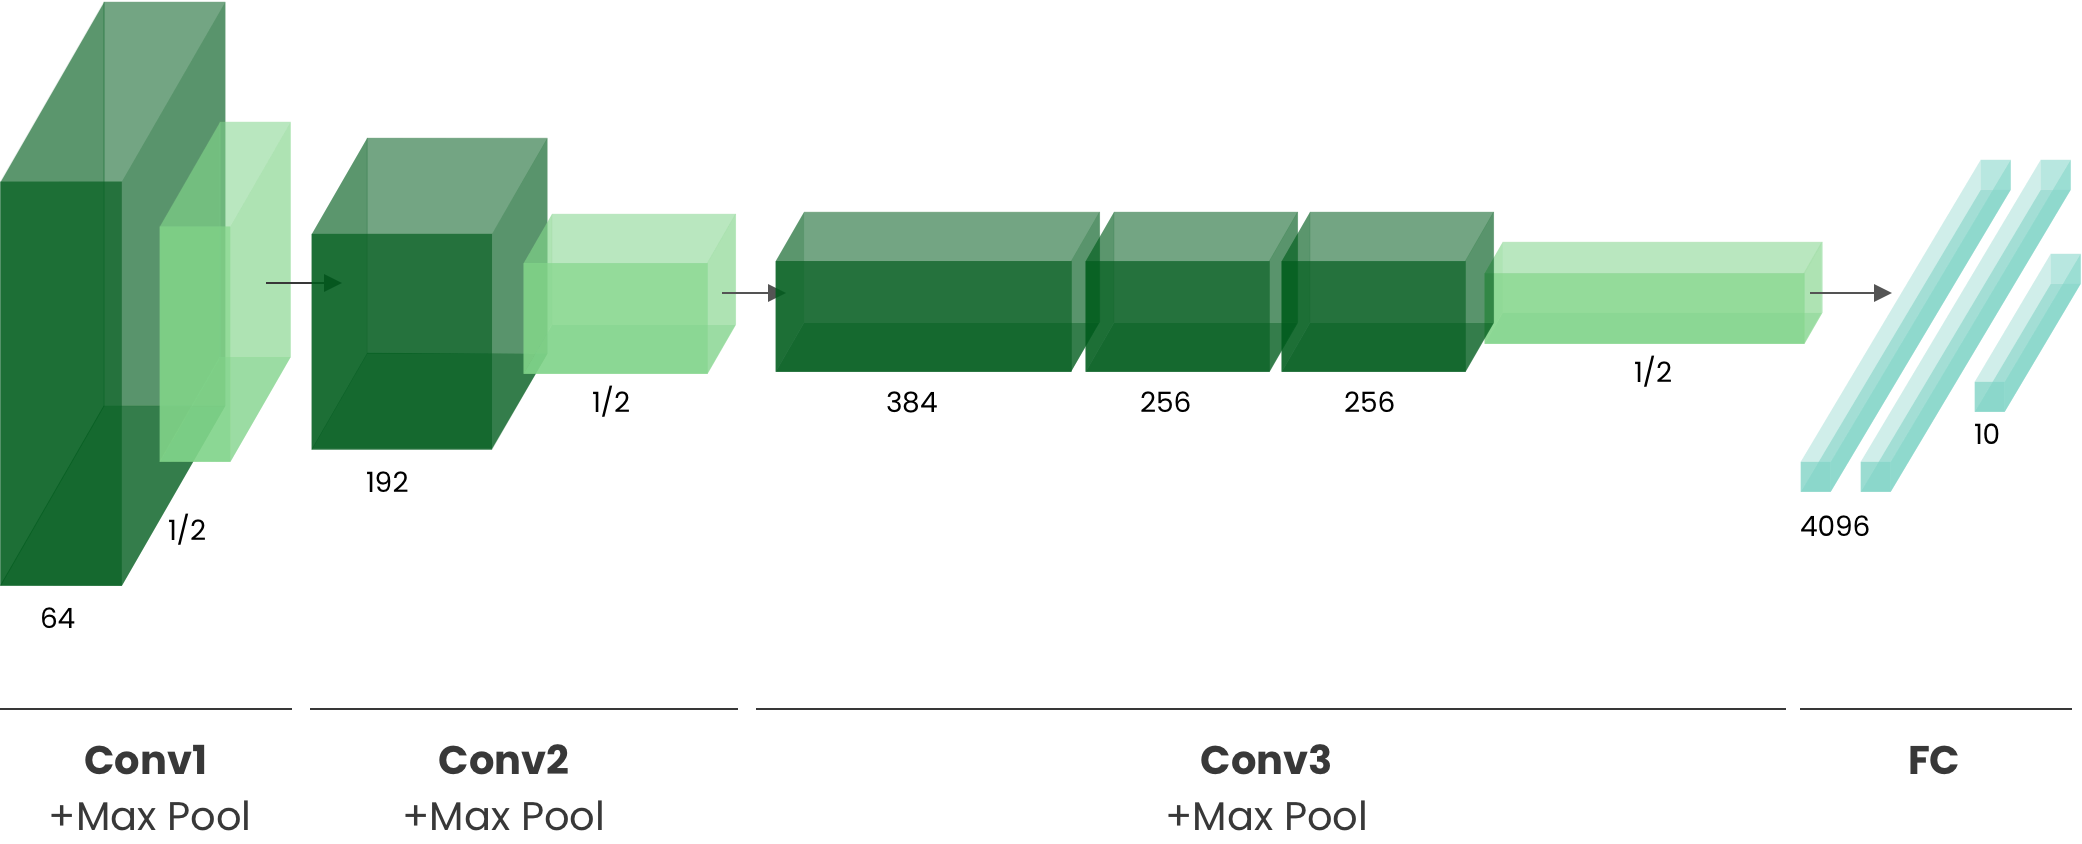
\includegraphics[width=0.95\textwidth]{./figures/alexnet.png}
  \end{center}
  \caption{\textbf{Convolutional Neural Network.} A schematic of a traditional
    convolutional neural network (CNN), designed for image classification (here:
    AlexNet~\cite{alexnet}). The network consists of a series of 2D
    convolutional layers, pooling layers and fully-connected layers, whose
  outputs are displayed as dark-green, light-green and blue boxes, respectively.
}
  \label{fig:cnn}
\end{figure}


CNNs are a type of neural network specifically designed to process visual
information. Traditionally, they are organised hierarchically and consist of
convolutional, pooling and fully-connected layers, as shown in
Figure~\ref{fig:cnn}. Convolutional layers are the core of CNNs and are
responsible for extracting features from the input. Each convolutional layer
consists of a set of filters, where each filter, sometimes called kernel $k$, is
a three-dimensional matrix of weights with dimensions $c_i \times h_k \times
w_k$, where $c_i$ is the number of channels in the input, and $h_k$ and $w_k$
are the height and width of the filter. Given an input $x$ with dimensions $c_i
\times h_i \times w_i$, a single convolutional filter $k$ produces a feature map
$z$ by sliding the filter across the spatial dimensions of the input, as shown
in Figure~\ref{fig:conv}a, and computing the convolution at each position
${i,j}$ (Equation: \ref{eq:2dconv}).

\begin{equation}
  z_{i,j} = \sum_{c=1}^{c_i} \sum_{m=1}^{h_k} \sum_{n=1}^{w_k} 
  k_{c,m,n} x_{c,i+m,j+n}
  \label{eq:2dconv}
\end{equation}

The output $z$ is a two-dimensional matrix, called feature-map. Within a single
convolutional layer, multiple filters are applied to the input, which results in
multiple feature-maps. After applying a non-linear activation to each feature
map, they are stacked along the channel dimension to form the output of the
convolutional layer, which is passed to the next layer. Pooling layers are often
interleaved with convolutional layers to reduce the dimensionality of feature
maps. The pooling operation is similar to convolution, as a kernel is slid over
the spatial dimensions of the input. However, instead of computing a weighted
sum, the pooling operation computes a statistic, such as the maximum (Max
Pooling) or average (Average Pooling), of the values in the kernel.

% why cnns work
CNNs have been found to work specifically well for data with a spatial structure
such as images, because convolutions model the inherent nature of images: While
a stand-alone pixel is not as informative, the value of a pixel in the context
of its neighbouring pixels is. This characteristic is naturally captured by the
convolution operation. Furthermore, in sliding filters across the input, they
can capture the same feature independently of its location in the image, which
makes CNNs invariant to translation. This is a desirable property for image
classification, as the location of features in an image may not be relevant for
the final classification.

% why cnns work
The first CNN-based architectures date back to the 1960s and have shown
successes in simple image classification tasks~\cite{lenet}. However, it was not
until 2012, when the CNN-based architecture AlexNet~\cite{alexnet} won the
ImageNet Large Scale Visual Recognition Challenge (ILSVRC)~\cite{imagenet}, that
CNNs arrived in the mainstream of computer vision. Since then CNNs have been
proposed in various different forms, mostly differing in the network's structure
and depth and the width and resolution of the filters. To this day, CNNs still
rank amongst the top performing methods in image classification benchmarks.

\begin{figure}
  \centering
  \begin{subfigure}[b]{0.49\textwidth}
    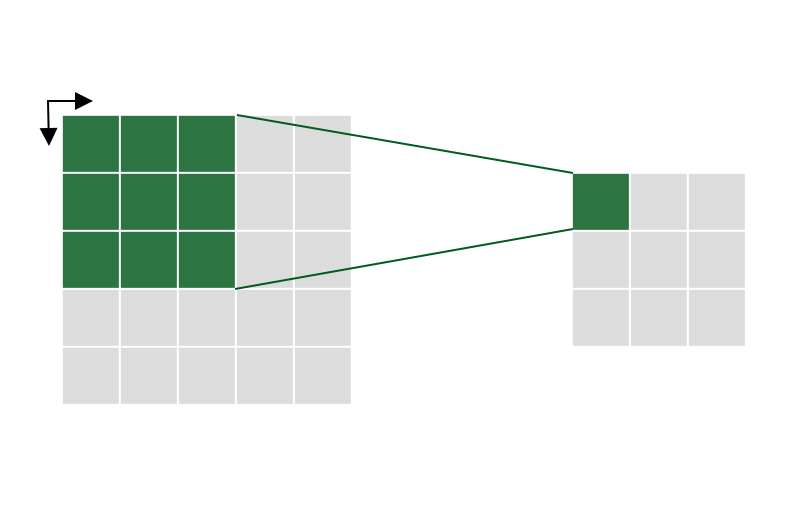
\includegraphics[width=\textwidth]{./figures/2d-conv.png}
    \caption{2D Convolution}
  \end{subfigure}
  \hfill
  \begin{subfigure}[b]{0.49\textwidth}
    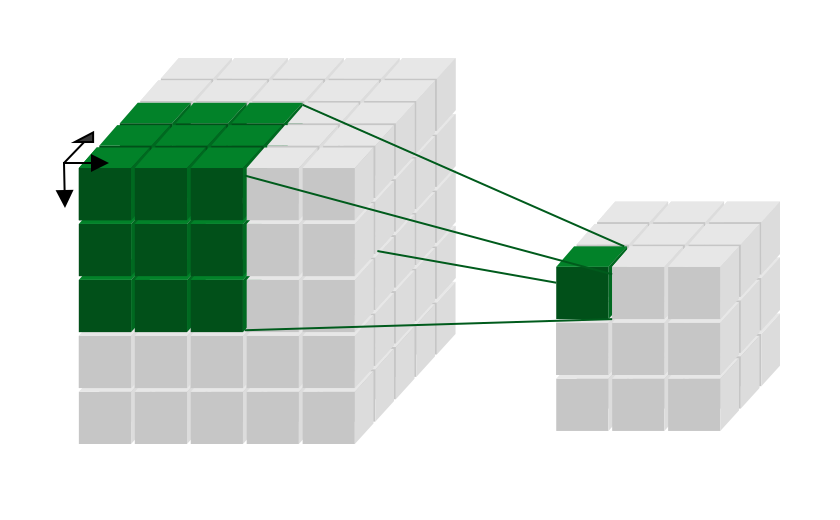
\includegraphics[width=\textwidth]{./figures/3d-conv.png}
    \caption{3D Convolution}
  \end{subfigure}
  \caption{
  \textbf{2D and 3D Convolution.} A simplified illustration striding of 2D and
  3D convolutional filters across an input. For visualisation purposes, a single
  channel is shown. A 2D convolutional filter (a) slides across the spatial
  dimension (height and width) of an input. A 3D convolutional filter (b) slides
across the spatio-temporal dimension (height, width, and time) of an input.}
  \label{fig:conv}
\end{figure}

\subsection{Video Classification}
\label{sub:video-classification}

Video classification can be seen as a generalisation of image classification:
Instead of assigning a label to a single image, video classifiers assign a label
$y$ or a sequence of labels $y_1, \ldots, y_t$ to a video sequence $x = (x_1,
\ldots, x_T)$, where $x_t$ is a frame of the video.

The difference is subtle, yet important, because it introduces a temporal
dimension to the task. It is generally assumed that the temporal dimension
is critical for video classification, because it provides additional
information about the video. For example, it might be difficult to determine
whether a person is running or walking from a single frame, but trivial given
the motion captured by a sequence of frames.

Motivated by the need for a powerful model to capture the semantic content of
video data and the success of CNNs in image classification, researchers have
started to apply CNNs to video classification~\cite{videocnn, i3d, c3d, x3d,
slowfast}, where the networks have access to the complex spatio-temporal
evolution of the video. Over the course of the last decade, various approaches
based on CNNs have been proposed that exhibit different connectivity patterns
for modelling the temporal dimension of the video~\cite{videocnn}.

% naive solution: single frame with averaging
A naive solution, which ignores the temporal dimension entirely, is to predict a
label for each frame and then average the predictions. Despite their simplicity,
these models have been shown to perform surprisingly well~\cite{videocnn}.
Different methods for aggregation have been proposed, such as
averaging~\cite{videocnn}, majority votes, or using a neural architectures, such
as recurrent neural networks (RNNs) to learn the importance of each
frame~\cite{lrcn} for the final prediction.

% model temporal dimension directly through 3d convolutions
CNN-based architectures that model the temporal dimension directly usually
leverage 3D convolutions~\cite{c3d, i3d}. 3D convolutions are a natural
extension of 2D convolutions, as defined in
Section~\ref{sub:image-classification}. Instead of sliding a convolutional
filter across the spatial dimension of the input (Figure~\ref{fig:conv}a), a
3D-convolutional filter slides across the spatio-temporal dimension of the input
(Figure~\ref{fig:conv}b), which produces feature maps in spatio-temporal space
that are learned jointly. 3D convolutions have been used in many different
variants. Architectures range from pure 3D convolution networks~\cite{i3d, c3d}
to hybrid architectures that combine 2D and 3D convolutions~\cite{x3d,
slowfast}. Overall, it can be summarised that, despite the introduction of
large-scale datasets for video classification~\cite{kinetics}, the research
field has not yet converged to a consensus about the best approach for video
classification.

\section{Data}

To train a deep learning model for indoor localisation, a labelled dataset is
required for training and evaluation. The following section describes the
collection, annotation and pre-processing of a novel video dataset tailored for
indoor localisation. Because the study investigates models trained on static
frames and sequences of frames, the pre-processing of the data differs and is
therefore described separately.

\subsection{Data Collection} % (fold)
\label{sub:data-collection}

% videos
The raw video data was collected from a single camera of a mobile device at a
frame rate of 30 FPS in high resolution ($2426\times 1125$). This process
yielded a set of videos $V = \{v_1, ..., v_n\}$, where each video $v_i$ is a
sequence of $k$ frames $f_1, ..., f_k$. Each frame $f_i$ is a RGB image with
dimensions $3 \times 2426 \times 1125$. Exemplary frames from the video clips
are shown in Figure~\ref{fig:frames} for illustration purposes.


\begin{figure}
  \begin{center}
    \includegraphics[width=\textwidth]{./figures/frames.png}
  \end{center}
  \caption{}
  \label{fig:frames}
\end{figure}

The mobile device was hand-held by a human agent while walking around the main
building of the Southern Campus of the Copenhagen University (Danish:
K\o{}benhavns Universitet, KU) in Copenhagen S, Denmark. The location was deemed
compatible with this study as it showcases distinctive learnable indoor features
(e.g. coloured walls, characteristic architectural structures, etc.), but also
challenges the model, for example, due to areas that are visually similar to
each other (like libraries and corridors). For the scope of this project, the
data collection was limited to the first two floors. 



% statistics of the data
A total of $n=53$ videos of varying length were recorded, with an average
duration of $\sim$57s, amounting to a total of $\sim$50 minutes of
footage, or an equivalent of $\sim$90K frames. 



\subsection{Data Annotation} % (fold)
\label{sub:data-annotation}

% labels
Each video $v_i$ is associated with a set of location labels $L = \{l_1, ...,
l_n\}$, where each location label $l_i$ identifies the location of the agent t
a specific time in the video. For the scope of this project 20 different
location labels were considered, which are identified by a descriptive name and
integer. Figure~\ref{fig:location-labels} shows the floor plan of the first two
floors of the building, where each location class is mapped to a coloured
region. The location labels were assigned in close correspondence to the
original floor plan. This, however, led to some classes being a lot larger than
others, which is likely to result in a class imbalance. Annotation was performed
manually by a single human agent. Because changes in the location labels only
occur at the transition of rooms, the annotation process was simplified by
annotating the starting and ending time stamps of a location label, which were
later pre-processed to frame-by-frame annotations. 

% figure
\begin{figure}
\centering
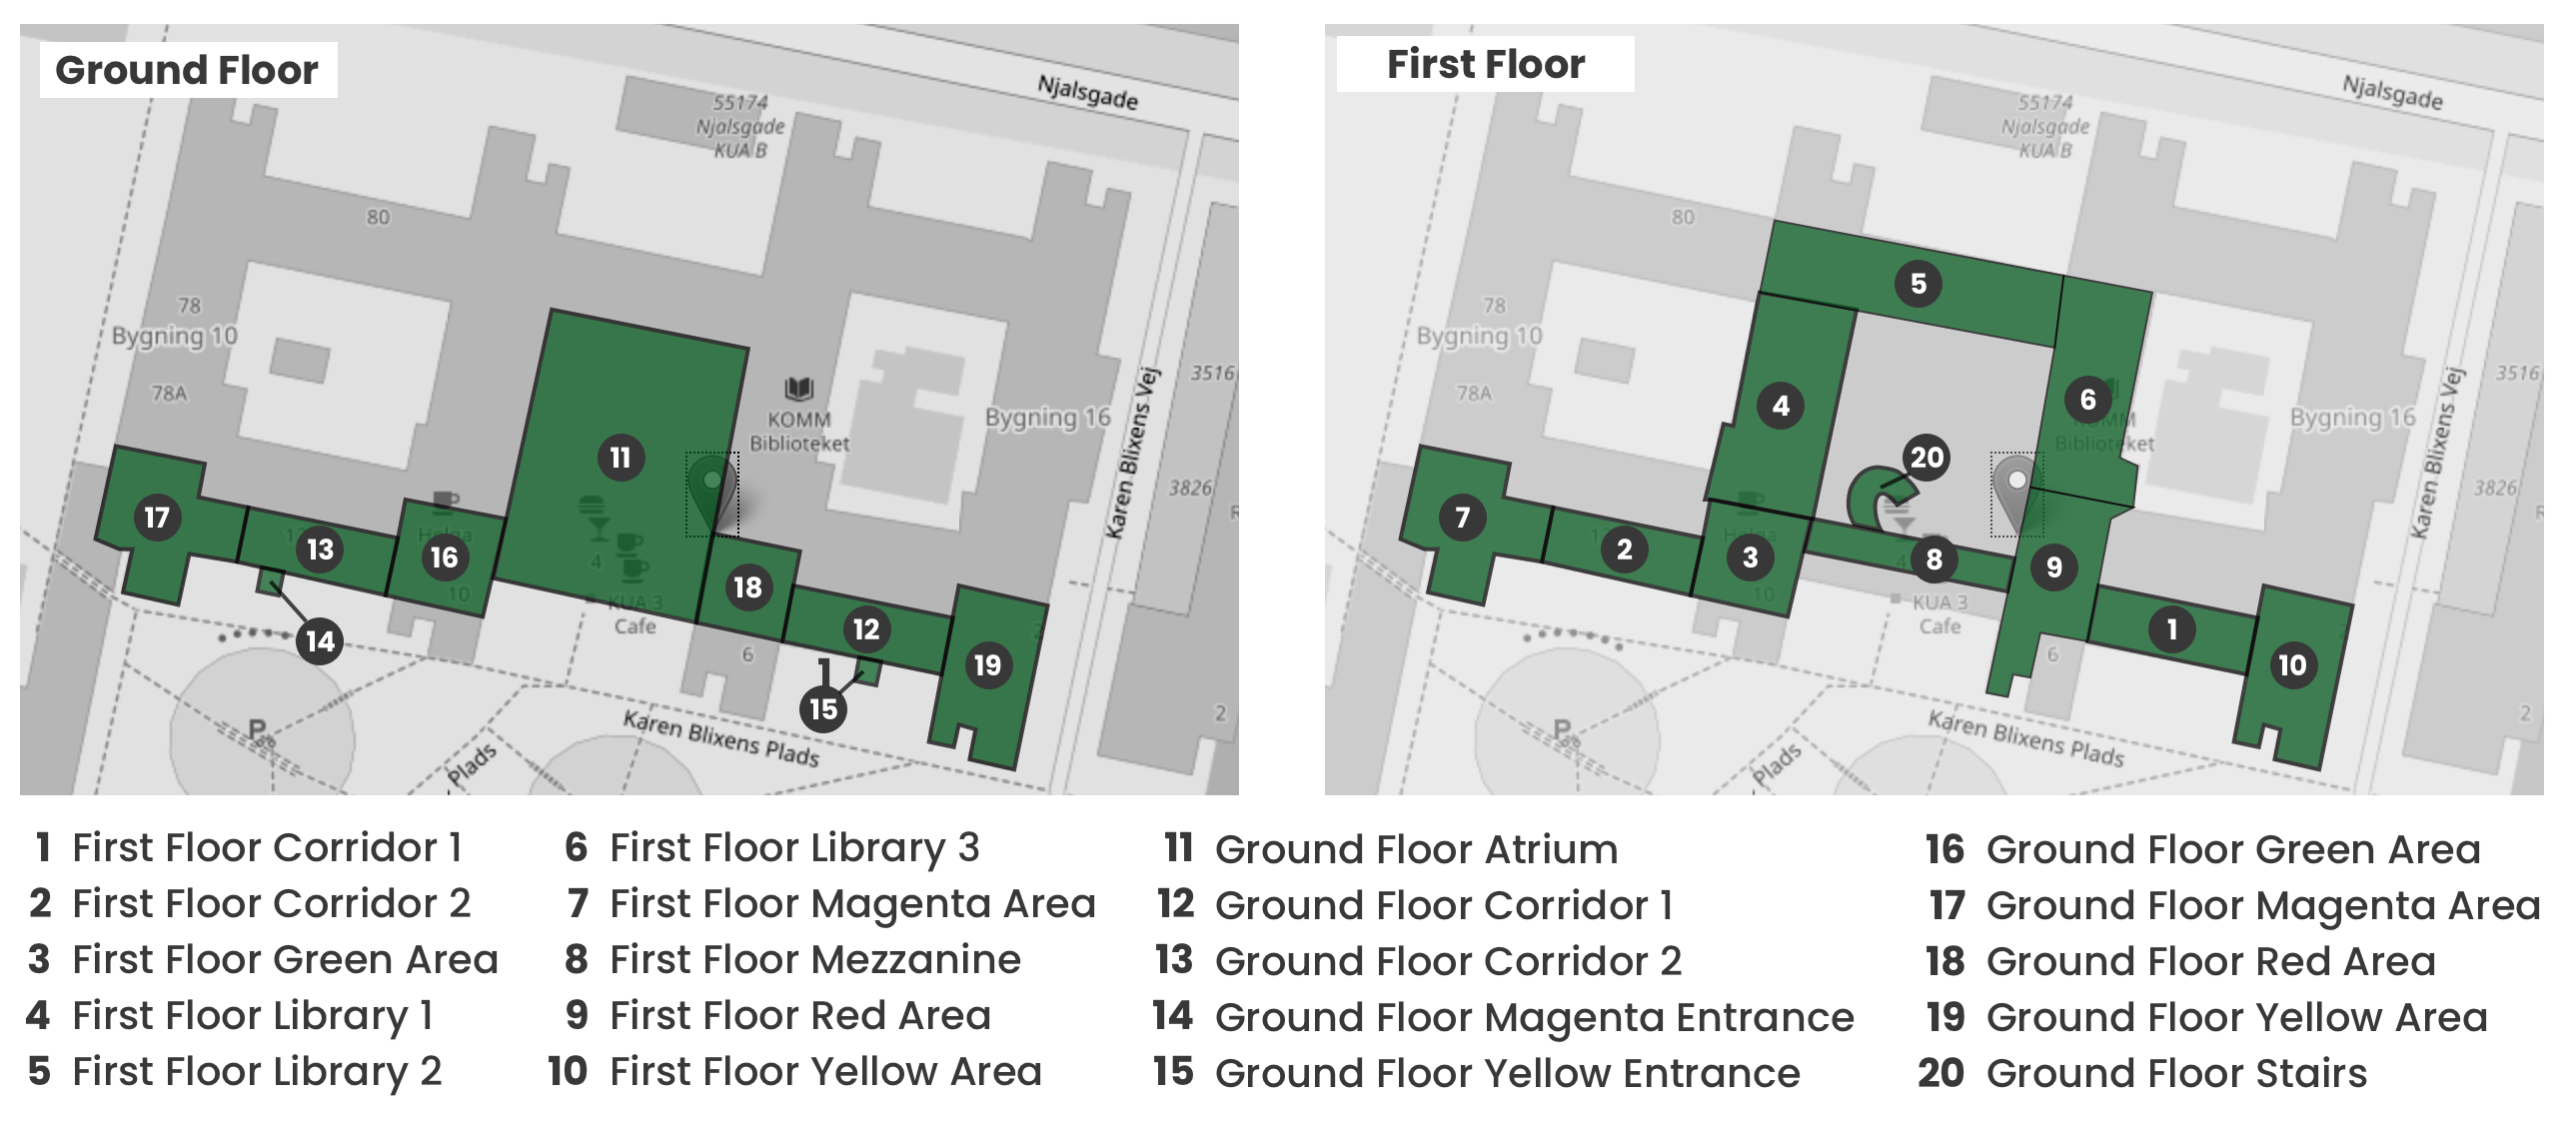
\includegraphics[width=\textwidth]{figures/location-labels.png}
\caption{
  \textbf{Location Labels.} The figure shows the floor plan for the ground floor
  (left) and first floor (right) of the main building of the Southern Campus of
  the Copenhagen University. The 20 location labels considered in this study are
  numbered and mapped to a coloured region on the floor plan.}

\label{fig:location-labels}
\end{figure}


% TODO: figure about the time of data collection (side-by-side, one where hue
%       denotes the split and the other where hue denotes the clips per day)

\subsection{Data Splits} % (fold)
\label{sub:data-splits}

Out of the total 53 videos that were recorded, 37 were used for training and 16
were used for testing. Importantly, the videos in the training split were
recorded in a single session, while the videos in the test split were recorded
on four separated days, in a span of two to four weeks after the training data
had been recorded. This was done to ensure that the models were tested against
unseen data, to more accurately assess their generalisation capabilities.
Indeed, the test data was recorded in different weather conditions, at different
times of the day, with different lighting conditions and, by pure chance, one of
the areas was repainted during the time between the recording of the training
and test data. With all these changes in mind, the test data is expected to be
as different from the training data, as it would be in a real-world scenario.


\subsection{Data Processing} % (fold)
\label{sub:data-processing}

% extraction of frames in training and testing
Single-frame classification models expect a single frame $f_i$ from a video
$v_i$ as input. Technically, all frames in a video $v_i$ could be used as input,
but because of the strong local correlation between adjacent frames, it was
hypothesised that models would overfit to the training data. For this reason,
and in an attempt to assimilate the single-frame and video datasets, frames from
a video $v_i$ were sampled at a sampling rate fixed $r_f$. The sampling rate is
not tied to the architecture of single-frame models and was therefore chosen
globally to be $r_f=5$ for the training split. This means that only every 5th
frame from the videos in the raw data split were used for training. A sampling
rate was not adopted for the testing split, in order to test the model on the
full set of frames.

% matching location
Matching the location labels to each of the extracted frames was
straight-forward. For each frame $f_i$ in a video $v_i$, the location label
$l_i$ was found as the label currently active at the time of the frame. This was
done by finding the location label $l_i$ that satisfied condition $t_{l_i} \leq
t_{f_i} \leq t_{l_{i+1}}$, where $t_{l_i}$ and $t_{f_i}$ are the time stamps of
the location label $l_i$ and frame $f_i$, respectively. This process yielded a
set of single-frame samples $D_F = \{(f_1, l_1), ..., (f_{n_f}, l_{n_f})\}$ with
$n_f=\sim 12K$ for the training split and $n_f=20K$ for the testing split.

\begin{figure}
\centering
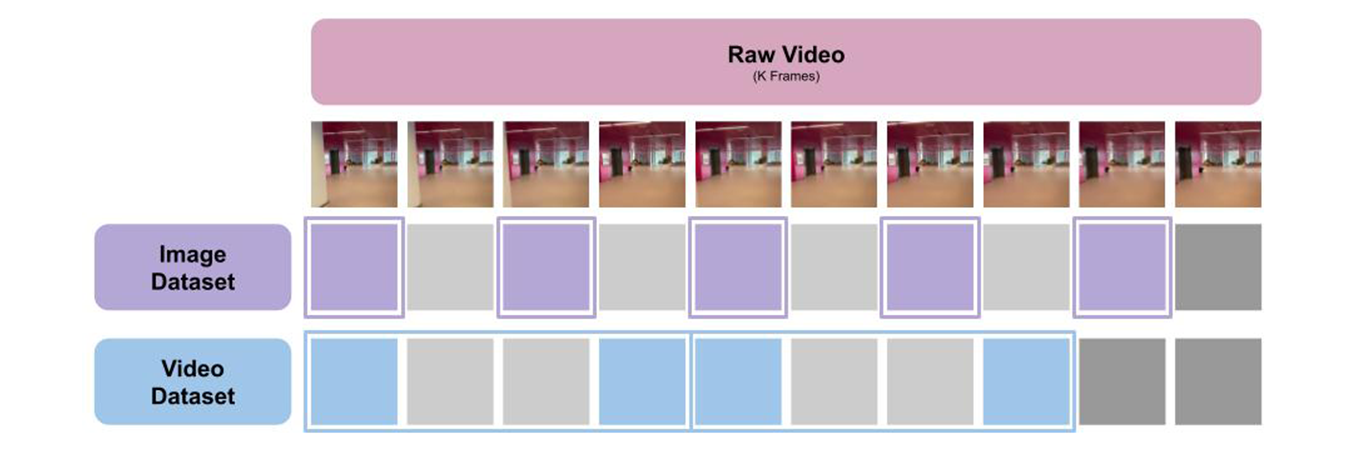
\includegraphics[width=0.95\textwidth]{figures/data-extraction.png}
\caption{
  \textbf{Data Extraction.} A raw video with $k=10$ frames is processed into
  $k_f=5$ frames for the single-frame dataset and $k_v=2$ clips for the
  video dataset. Samples for each dataset type are indicated by a
  surrounding box. Frames are sampled at a rate of $r_f=2$ for the
  single-frame dataset and $r_v=3$ for the video dataset. A clip contains
  $s_v=2$ frames. Frames are colour-coded in correspondence to the dataset
  they belong to (single-frame dataset in purple and video dataset in blue),
  if they are sampled to the respective dataset. Discarded frames are
  coloured in grey (light-grey for within video frames, dark-grey for
  trailing frames).}
\label{fig:data-extraction}
\end{figure}


A video classification model expects a single clip $c_i$ as input, which is a
fixed-sized sequence of $s_v$ frames sampled from a video $v_i$ at a sampling
rate $r_v$. For this reason, the video classification dataset is constructed by
extracting clips from the videos in the raw data split. Clips are extracted in
uniformly spaced intervals. Within this study only non-overlapping clips were
considered, meaning that in a single clip $c_i$, the location label $l_i$ is the
same for all frames $f_i \in c_i$. This is a simplification of the problem, as
it is possible for a person to move from one location to another within a single
clip, but was found more compatible with existing video classification
architectures. In reality, the simplification is viable, because during the
relatively small clip duration of $\sim 2$s, transitions between locations only
occur in a small subset of clips.

Because clips do not overlap multiple location labels, each clip $c_i$ can be
associated with a single location label $l_i$. The location label $l_i$ is found
as the location label present during the entire time span of the clip. This
process yielded a set of clip-location samples $D_V = \{(c_1, l_1), ...,
(c_{n_v}, l_{n_v})\}$.

% TODO: add resizing and standardisation of channels

% \subsubsection{Dataset Comparison} % (fold)
% 
% The extraction of clips and frames for video and single-frame classification
% models, respectively, is illustrated in Figure~\ref{fig:data-extraction}. It
% shows that, despite the common raw data source, the frames considered in the two
% datasets may not be the same. This is because of different sampling rates and
% because adjacent clips reset the sampling rate. 
% 
% Assuming a single video $v_i$ with $k$ frames, the number of frames $k_f$ that
% can be sampled from $v_i$ at a sampling rate $r_f$ is $k_f = \lfloor k / r_f
% \rfloor$. The number of clips $k_v$ that can be sampled from $v_i$ at a sampling
% rate $r_v$ is $k_v = \left\lfloor \frac{k}{r_v \cdot s_v} \right\rfloor \cdot
% s_v$. 
% 
% It becomes clear, that
% 
% 
% \[
%   \left\lfloor \frac{k}{r_v \cdot s_v} \right\rfloor \cdot s_v \approx
%   \left\lfloor \frac{k}{r_f} \right\rfloor, \quad \text{if} \quad r_v = r_f.
% \]
% 
% For this reason, the sampling rate $r_f$ for the single-frame dataset was chosen
% to be an as close as possible to the sampling rates of video classifiers. As
% multiple video classifiers considered in this study have different sampling
% rates ranging from $2$ to $8$, the sampling rate $r_f$ was chosen to be $5$.
% 
% This choice does not ensure that the two datasets are identical, but it ensures
% that the total number of frames in each dataset is similar, which means that
% all models visit similarly many frames during training.
% 
% Furthermore, it was hypothesised, that due to the large number of total frames
% and strong local correlation between adjacent frames, the two datasets are
% sufficiently similar to allow for comparison between the two model types.

% TODO: add statistics about nf and nv (number of frames and clips in train
% and test)

% subsection data-preprocessing (end)

\section{Methodology} % (fold)
\label{sec:methodology}

To assess the capabilities of different deep learning models, the study follows
a standardised methodology. First, a self-gathered dataset is collected,
annotated and preprocessed according to the specification of the problem
setting. Next, a series of deep learning models are selected and trained under
constant conditions on the same dataset and evaluated using a collection of
commonly used metrics for performance and efficiency. Finally, the results are
analysed in order to discuss the applicability of deep learning models for
indoor localisation.

One major distinction between the different models is whether or not they
operate on a single-frame or a sequence of frames. Because this distinction
impacts all steps of the study, from data processing to model evaluation, the
following two different problem settings are distinguished throughout the entire
study:

\begin{enumerate}

\item \textbf{Single-frame classification}: Given a continuous stream of frames,
  the task is to classify each frame individually.

\item \textbf{Video classification}: Given a continuous stream of frames, the
  task is to classify fixed-sized clips of the video.

\end{enumerate}


\subsection{Models} % (fold)
\label{sub:models}


Following the literature on single-frame and video classification tasks, twelve
different models were trained and evaluated in this work. Following the
distinction made in Section~\ref{sec:methodology}, the models are grouped into
single-frame and video classification models. 

Table~\ref{tab:model-overview} gives a comprehensive overview of all models. The
table shows the release year, the sampling rate $r_f$ for single-frame
classification models and the sampling rate $r_v$ and clip size $s_v$ for video
classification models. The table also shows the input size, the number of
parameters and the number of floating point operations (FLOPs) for a single
forward pass. Finally, the table shows the Top-1 accuracy on the ImageNet
dataset~\cite{imagenet} for single-frame classification models and the Top-1
accuracy on the Kinetics dataset~\cite{kinetics} for video classification as an
indicator of the model's performance on a generic classification task.

The following section briefly describes the main architectural features of each
model.

% mention pre-processing

\begin{table}
  \centering
  \caption{
    \textbf{Model Overview.} The table shows all models that were evaluated in
    this work. The models are split into two categories: single-frame models and
    video models. For each model, the table reports the release year (Release),
    the frame rate (Rate) of the training data, the number of frames per clip
    (F/C; \textit{only applicable to video classifiers}), the spatial resolution
    (Size) of the input images, the number of parameters in millions (Params),
    the number of floating point operations in billions (FLOPs) and the
    benchmark Top-1 accuracy (Acc\@1) on ImageNet~\cite{imagenet} for
    single-frame classification models and the Top-1 accuracy on the
    Kinetics~\cite{kinetics} dataset for video classification models. The table
    is sorted by release date within each group.
  }
  \begin{tabular}{cllllllll}
    \toprule
    & \multirow{2}{*}{\textbf{Model}} 
    & \bfseries Release & \bfseries Rate & \bfseries F/C & \bfseries Size &
    \bfseries Params & \bfseries FLOPs & \bfseries Acc@1 \\
    & & (Y) & ($r_f$/$r_v$) & ($s_v$) & ($h$, $w$) & (M) & (G) & (\%) \\
    \midrule
  \multirow{8}{*}{\rotatebox[origin=c]{90}{Single-Frame}} 
  & AlexNet~\cite{alexnet} & 2012 & 5 & - & 224 & 61.1 & 0.71 & 56.52 \\
  % & GoogLeNet~\cite{googlenet} & 2014 & 30 & - & 256 & 6.6 & 1.5 & 69.78 \\
  & ResNet18~\cite{resnet} & 2015 & 5 & -  & 224 & 11.7 & 1.81 & 69.76 \\
  & ResNet50~\cite{resnet} & 2015 & 5 & -  & 224 & 25.6 & 4.09 & 76.13 \\
  & DenseNet 121~\cite{densenet} & 2016 & 5 & - & 224  & 7.0 & 2.88 & 74.43 \\
  & MobileNet V3~\cite{mobilenetv3} & 2019 & 5 & - & 224  & 3.5 & 0.32 & 71.88 \\
  & ViT-B-16~\cite{vit} & 2020 & 5 & - & 224  & 86.7 & 17.56 & 81.07 \\
  & EfficientNet V2 S~\cite{efficientnetv2} & 2021 & 5 & - & 224  & 21.5 & 8.37 & 84.23 \\
  & ConvNext Tiny~\cite{convnext} & 2022 & 5 & - & 224  & 28.2 & 4.46 & 82.52 \\
  \midrule
  \multirow{4}{*}{\rotatebox[origin=c]{90}{Video}}
  & R(2+1)D~\cite{r2plus1d} & 2018 & 4 & 16 & 182 & 28.11 & 76.45 & 76.01 \\
  & Slow R50~\cite{slowfast} & 2018 & 8 & 8 & 224 & 32.45 & 54.52 & 74.58 \\
  & SlowFast R50~\cite{slowfast} & 2018 & 8 & 8 & 224 & 34.57 & 65.71 & 76.94 \\
  & X3D S~\cite{x3d} & 2020 & 6 & 13 & 182 & 3.5 & 2.96 & 73.33 \\
  \bottomrule
  \end{tabular}
  \label{tab:model-overview}
\end{table}

\subsubsection{Single-Frame Classifiers} % (fold)

\textbf{Alexnet}~\cite{alexnet} is a convolutional neural network that was
introduced by Krizhevsky \textit{et al.} in 2012. It was the first deep neural
network to win the ImageNet Large Scale Visual Recognition
Challenge~\cite{imagenet} and is considered to be one of the first successful
applications of deep learning to image classification. Architecturally, it
consists of five convolutional layers with occasional max-pooling layers in
between, followed by three fully connected layers, as illustrated in
Figure~\ref{fig:alexnet}.

\begin{figure}
  \centering
  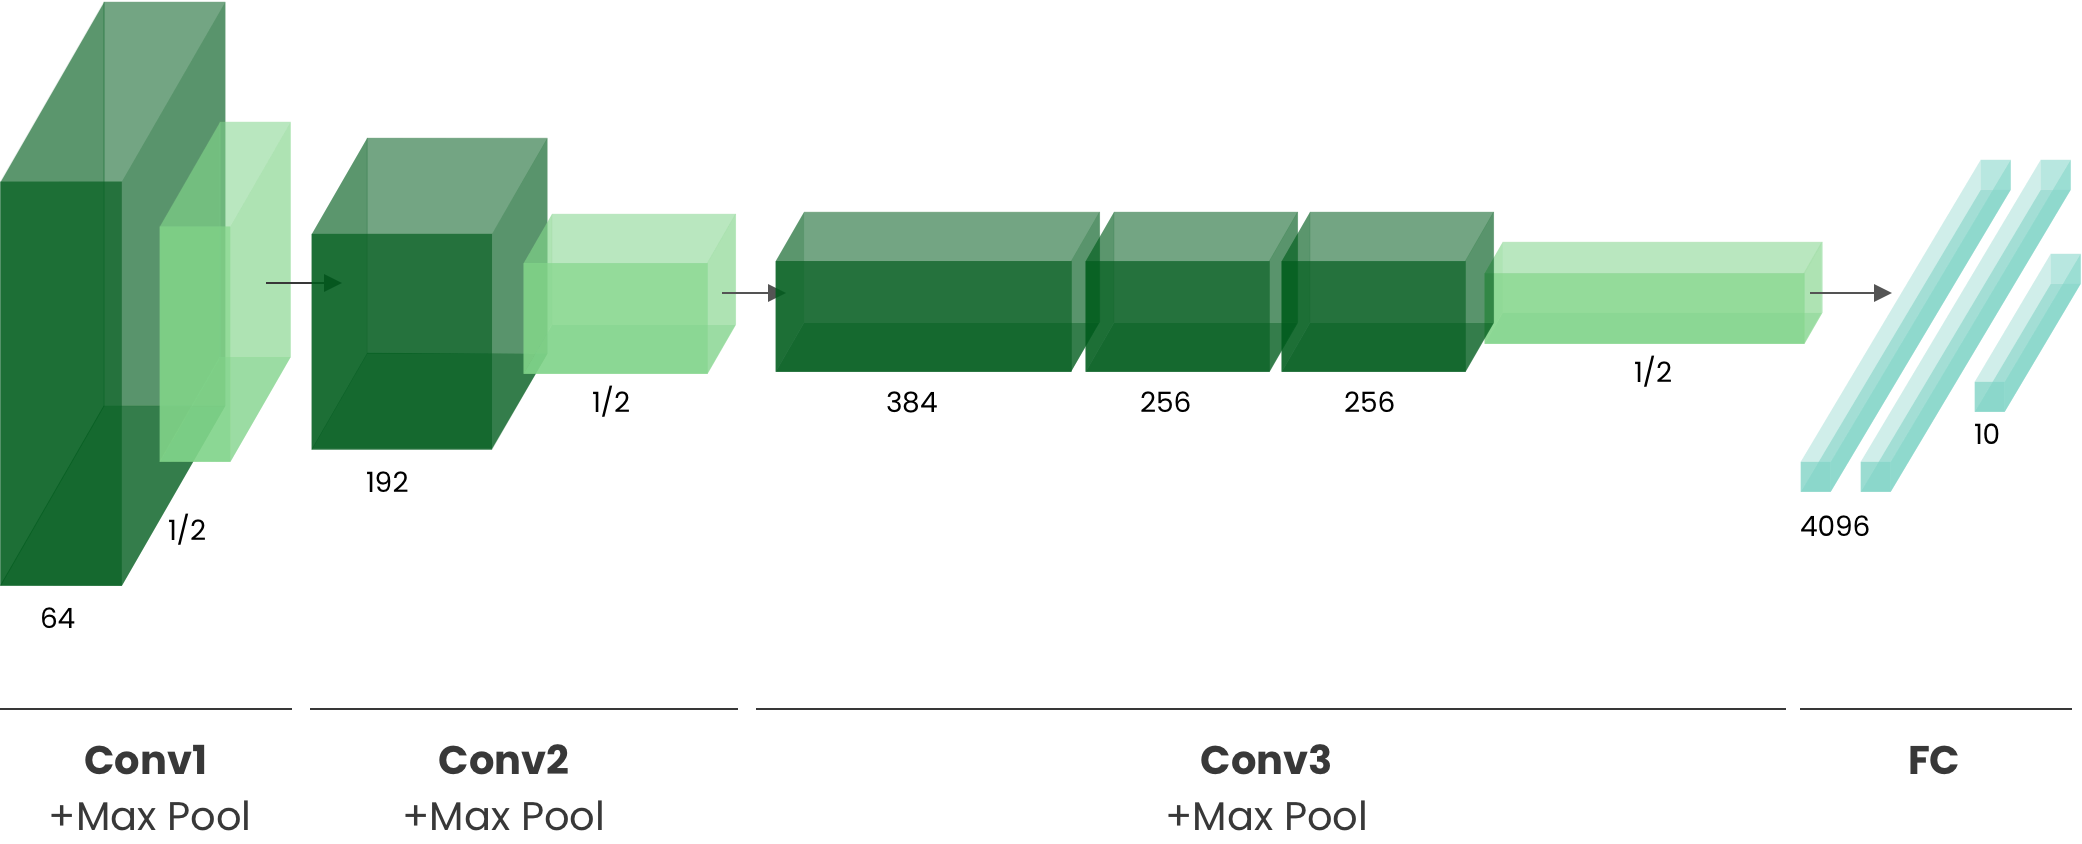
\includegraphics[width=\textwidth]{./figures/alexnet.png}
  \caption{\textbf{AlexNet Architecture.} An illustration of the architecture of
    AlexNet~\cite{alexnet}. Each box represents the output of a layer.
    Dark-green boxes are outputs of convolutional layers, light-green boxes are
    outputs of max-pooling layers and blue boxes are outputs of fully connected
    layers. The number of channels is denoted below each convolutional layer.
    Spatial downsampling is only performed by the first convolutional layer and
    all pooling layers. The downsampling factor is denoted below the pooling
    boxes.
  }
  \label{fig:alexnet}
\end{figure}

% \textbf{GoogLeNet} is a convolutional neural network that was introduced by
% Szegedy et al.~\cite{googlenet} in 2014. At its core, it is based on Inception
% modules, which allow the network to choose between multiple convolutional
% filter sizes in each block. Each inception module consists of 4 parallel
% convolutional layers, whose outputs are concatenated along the channel
% dimension. This advancement allowed the Google Team to significantly reduce
% the number of parameters in the network and win the ImageNet Large Scale
% Visual Recognition Challenge~\cite{imagenet} in 2014.

After the success of AlexNet, the speed of research in the field of deep neural
networks significantly picked up. Networks with increasing depth, such as
VGG~\cite{vgg}, were found to perform better, but led to new research problem:
As information about the input or gradient passes through many layers, it can
vanish during gradient-descent based learning, leading to a stagnation during
training. The phenomenon of "vanishing gradients" was visible in larger training
errors for deeper networks, and coined the "degradation" problem~\cite{resnet}. 

The \textbf{ResNet}~\cite{resnet} architecture is considered a cornerstone of
modern deep learning history as it introduced the concept of residual
connections. In a residual subnetwork of $L$ layers $H_l$, the output $x_l$ is
computed as the sum of the input to the subnetwork $x_{l-1}$ and the output of
the subnetwork $H_l(x_{l-1})$, i.e. $x_l=x_{l-1}+H_l(x_{l-1})$. The introduction
of this identify mapping to the output of the subnetwork was shown to facilitate
signal propagation in forward and backward paths, and, in connection with batch
normalisation~\cite{batchnorm}, allowed to train networks of unprecedented
length. The original paper introduced several architectures with different
depths, but in this work only ResNet18 and ResNet50, with 18 and 50 layers
respectively, are considered.

\begin{figure}
  \centering
  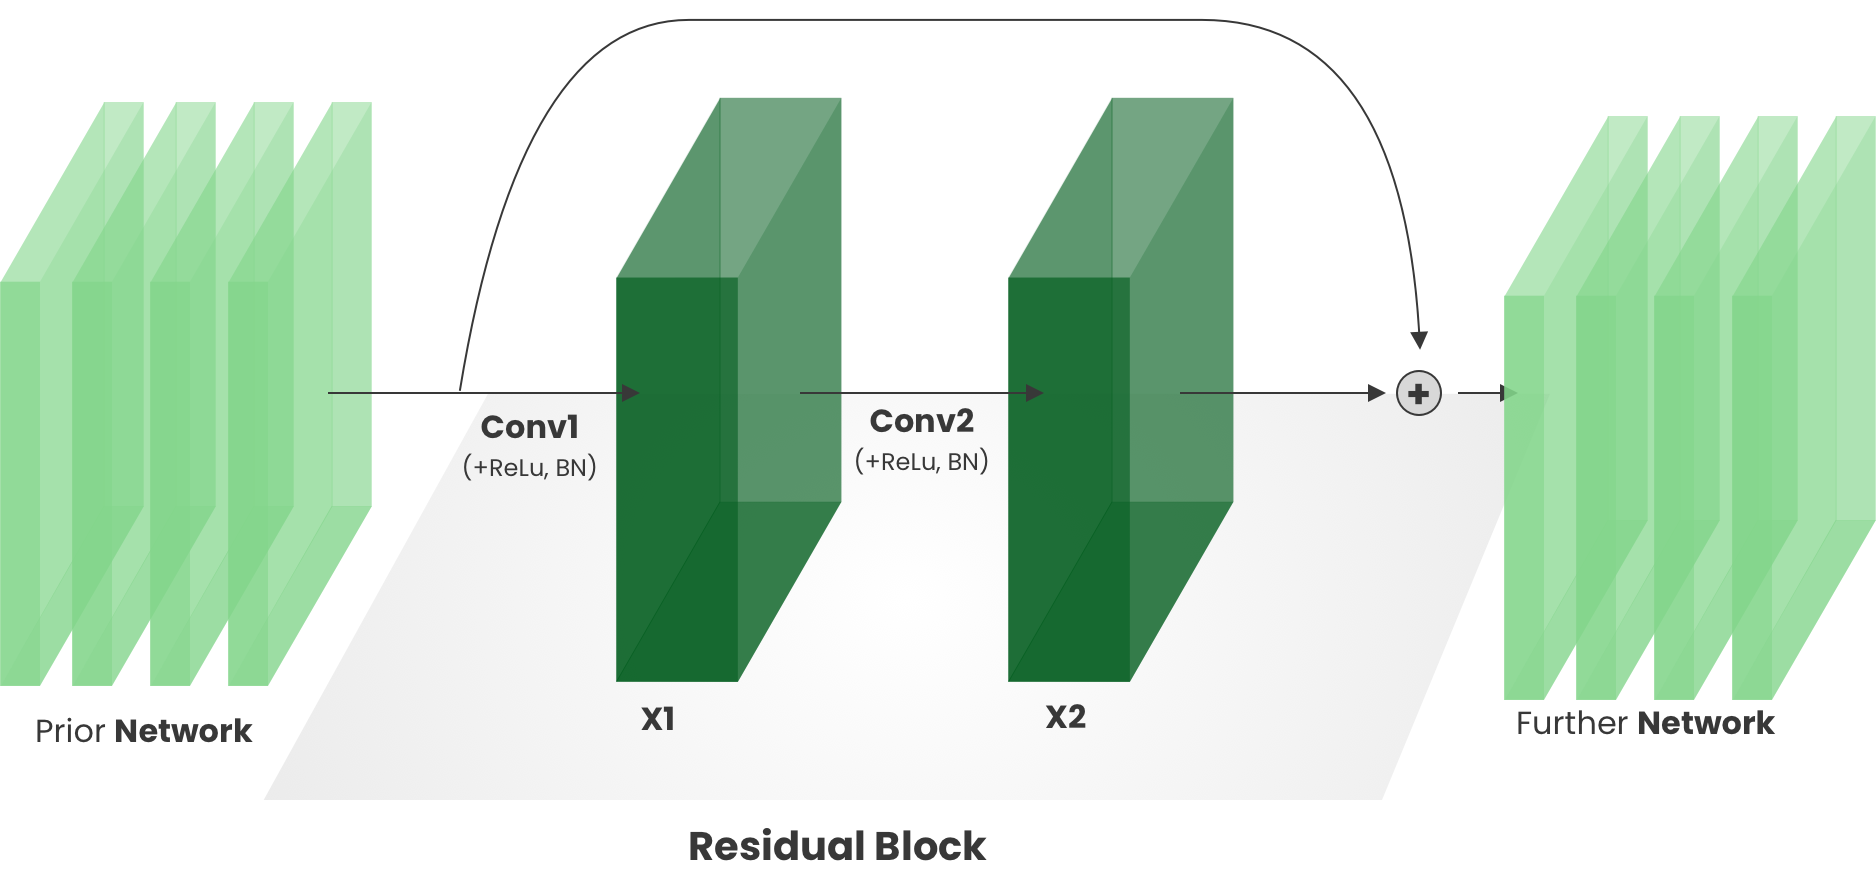
\includegraphics[width=0.8\textwidth]{./figures/resnet.png}
  \caption{\textbf{Residual Connection.} An illustration of a generic residual
  block, as defined by He \textit{et al.}~\cite{resnet}. A subnetwork of $L=2$ layers
  (consisting of convolution, batch normalization and ReLU layers) is applied to
  an input $x_0$. The first layer produces an output $x_1$, and the second layer
  an output $x_2$. The output of the residual block is given by $x_2+x_0$
  through the skip connection.
  }
  \label{fig:residual-connection}
\end{figure}

\textbf{DenseNets}~\cite{densenet} extend the idea of residual connections. At
the core of the DenseNet architecture is the concept of "dense blocks": Similar
to a residual block, it is a subnetwork of $L$ layers denoted as $H_l$. Unlike
the residual block, each layer in the dense block receives the concatenation of
all preceding layer outputs as an input, such that $x_l = H_l([x_0, x_1, \dots,
x_{l-1}])$. Dense blocks are compute intensive, but the strong connectivity
between layers support feature reuse, which allowed the architecture to be
shallower than predecessors. Again, the authors introduced several architectures
with different depths. Here, only DenseNet 121 is considered.

\begin{figure}
  \centering
  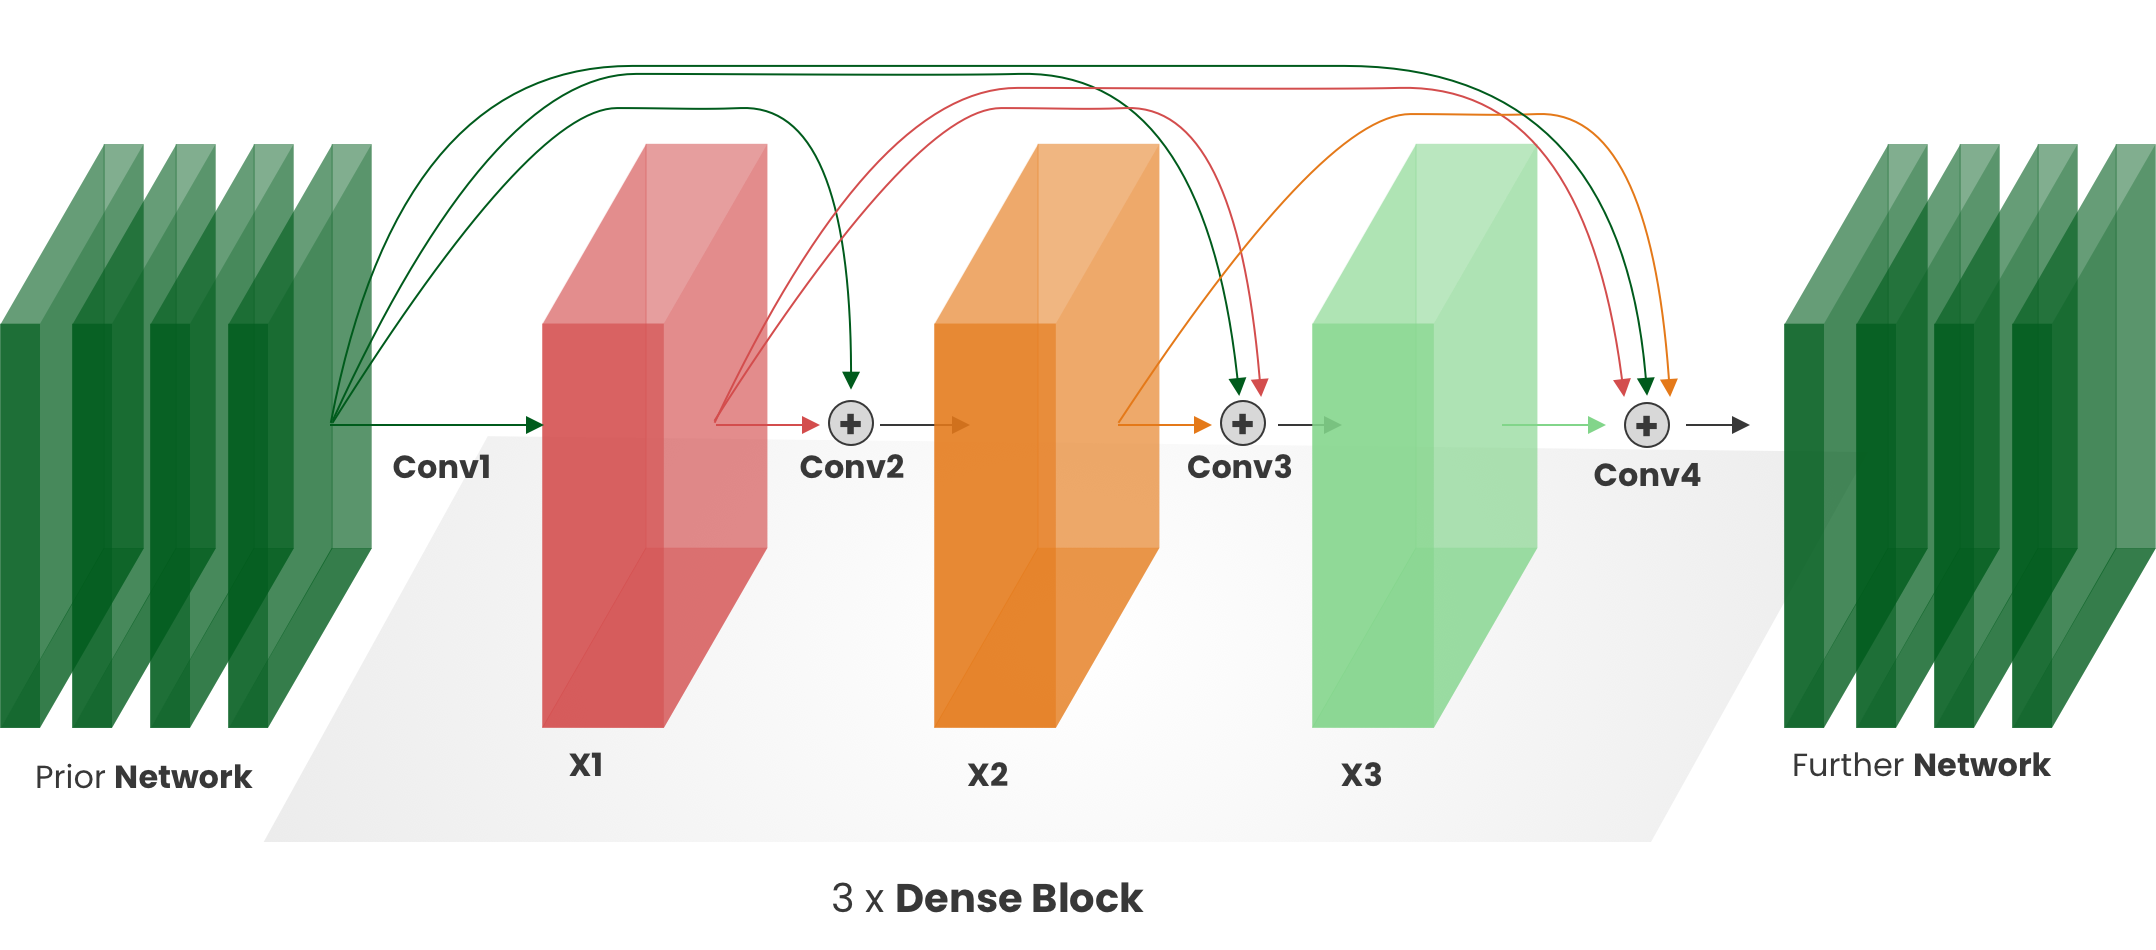
\includegraphics[width=.8\textwidth]{./figures/densenet.png}
  \caption{\textbf{Dense Block.} An illustration of a generic dense block, as
    defined by Huang \textit{et al.}~\cite{densenet}. A subnetwork of $L=4$ layers
    (consisting of convolution, batch normalization and ReLU layers) is applied
    to an input $x_0$. The $i$-th layer produces an output $x_i$. The input to
    the $i$-th layer is the concatenation of the output of all previous layers,
    so $H_i(x_i) = H_i([x_0, x_1, \dots, x_{i-1}])$. The final output of the
    denseblock is the concatenation of the output of all layers, so $x_4 = [x_0,
  x_1, x_2, x_3]$. }
  \label{fig:denseblock}
\end{figure}

\textbf{MobileNet V3}~\cite{mobilenetv3} is the third iteration of the MobileNet
architecture, which was introduced by Howard \textit{et al.} 2019. The main contribution
of MobileNets are so-called depth-wise separable convolutions. A depth-wise
separable convolution factorises a regular 2D convolution into two separate
steps: First, a single 2D filter is applied to each input channel separately,
and then a 1x1 convolution is applied to the output of the previous step. This
architectural change makes MobileNets significantly more efficient with only
minor performance losses, which made them popular for application on low-compute
devices, like mobile phones. MobileNet V3 is the most recent iteration of the
architecture, and its smallest variant, MobileNet V3 Small, is used in this
work.

\textbf{EfficientNet V2}~\cite{efficientnetv2}, proposed by Tan \textit{et al.}
in 2021, is searching for a compute-optimal CNN architecture. The main finding
of the paper is a scaling law, which states that for a given baseline network,
e.g. scaling up a network's depth, width and resolution with a constant factor
leads to improved performance and efficiency. In the original paper the authors
scale up previous state-of-the-art models like ResNet and MobileNet, which
showcase state-of-the-art performance, which make up a new family of models
called EfficientNets. Here, EfficientNet V2 S is used, which is the smallest
variant of the EfficientNet V2 family.

With the ground-breaking paper "Attention is all you need"~\cite{transformer},
Vaswani \textit{et al.} introduced the Transformer architecture in 2017.
Although being initially designed for machine translation, the architecture was
quickly adapted to other tasks in the domain of natural language processing,
superseding previous state-of-the-art models on various benchmarks. 

In 2020, \textbf{Vision Transformer}~\cite{vit} was introduced as one of the
first Transformer-based model adapted for the computer vision tasks. The main
contribution of the model is the patch embedding mechanism, which overcomes the
architectural mismatch between the two-dimensional input of images and the
one-dimensional input of Transformer architectures. Dosovitskiy \textit{et al.}
propose to split a two-dimensional image into a sequence of fixed-sized
patches, which are then flattened and embedded into a sequence of "tokens".
Together with positional encodings for the position of the patch in the original
image, this sequence of tokens can be fed into a regular Transformer
architecture. The authors introduce several configurations of the architecture.
In this work, the base Vision Transformer, ViT-B-16, which is among the smaller
variants of the model is used.

Since then, many variants of the Vision Transformer have been proposed. They
either decrease the computational complexity of the architecture~\cite{deit,
vitlite}, or improve the performance by recovering some of the inherent
architectural advantages of convolutional neural networks~\cite{swin}. However,
these architectures are not considered in this work.

Finally, \textbf{ConvNext}~\cite{convnext} is one of the most modern
convolutional neural network architectures considered in this work and was
proposed by Liu \textit{et al.}~\cite{convnext} in 2021. Against the trend of
Transformer-based architectures in computer vision tasks, ConvNext is a pure
convolutional architecture. ConvNext uses the ResNet 50~\cite{resnet}
architecture as a baseline and performs gradual modernisation steps, ranging
from different optimisation algorithms, filter dimension to network depth and
width. The authors show that the resulting convolutional architecture is
competitive with the Transformer-based architectures, and coined in ConvNext.

\subsubsection{Video Classifiers} % (fold)

Early attempts of using 3D convolutional filters for video classification
tasks~\cite{i3d, c3d} show potential for modelling the temporal dimension of
video data. However, the authors also show that simple single-frame models
perform surprisingly well, and that the temporal dimension only provides
marginal gains. This finding and the fact that one would expect the temporal
information and motion patterns that emerge in sequences of images to be
important for video motivated Tran et. al to investigate different architectural
designs for video classification tasks. They contrast regular 3D convolution,
mixed 2D and 3D convolution, 3D convolution and 3D convolution with factorised
filters, which they coin \textbf{R(2+1)D}~\cite{r2plus1d}. They find that the
R(2+1)D architecture improves the performance on the Kinetics dataset by a
noticeable margin. 

In the same year, Feichtenhofer \textit{et al.}~\cite{slowfast} proposed
\textbf{SlowFast}~\cite{slowfast}, which introduces a two-stream architecture
for video classification tasks. SlowFast has two separate pathways for
processing video data. The first pathway, the slow pathway, processes the video
data at a low frame rate, which allows it to capture the spatial information of
the video data. The second pathway, the fast pathway, processes the video data
at a high frame rate, which allows it to capture the temporal information of the
video data. The authors show that the combination of the two pathways improves
the performance over single-stream architectures. In this study, both the
single-stream slow architecture \textbf{Slow R50} and the two-stream
architecture \textbf{SlowFast R50} are considered.

Finally, the \textbf{X3D} architecture reviews the design choices of previous
architectures that were proposed. The authors find that previous approaches
differ mainly by varying the temporal dimension (frame rate and number of
frames) and the spatial dimension (resolution, depth and width of filters).
Jointly studying the effects of scaling the temporal and spatial dimensions, the
authors propose a family of architectures that gradually scales up the depth,
width and resolution of the network, while keeping the computational complexity
constant. In this work, the smallest variant of the X3D family, X3D S,
is used.

% subsection models (end)

\subsection{Training} % (fold)
\label{sub:training}

All models were implemented using the deep learning framework \texttt{PyTorch}.
The model architectures were taken from the \texttt{Torchvision} and
\texttt{Pytorchvideo} libraries and initialised with the default pre-trained
weights provided by the libraries. Single-frame and video classifiers were
pre-trained on the ImageNet~\cite{imagenet} and Kinetics~\cite{kinetics}
datasets, respectively. Fine-tuning was performed remotely on the
high-performance cluster (HPC; Appendix~\ref{sub:machine-specs}) of the IT
University of Copenhagen using GPU-accelerated training. 

All models were optimised to minimise the cross-entropy loss function
$\mathcal{L}$ (Equation \ref{eq:cross-entropy}), 

\begin{equation}
  \mathcal{L}(\hat{\mathbf{y}},\mathbf{y}) = -\sum_{i=1}^{L} \mathbf{y}_i
  \log(\hat{\mathbf{y}}_i) \quad ,
  \label{eq:cross-entropy}
\end{equation}

% TODO: compare to pytorch cross-entropy loss (is it the same? what is the
% difference to nll?)

% TODO: models are all fine-tuned


where $\hat{\mathbf{y}}$ is the predicted probability distribution over the $L$
location labels, and $\mathbf{y}$ is the one-hot encoded ground truth location
label for a single frame or video. The function penalises the model for
predicting a low probability for the ground truth label. For the models to learn
the relationship between frames/ clips and location labels, the gradient of the
loss function with respect to all model parameters is computed and
AdamW~\cite{adamw}, the de facto standard optimiser for deep learning models, is
employed to update the model parameters at a constant learning rate of
$10^{-4}$. No learning rate warm-up or scheduling was performed during training.

Mini-batch training was used for all models with a batch size of 16 for
single-frame models and 4 for video classification models due to memory
constraints. Because of the high computational complexity of 3D convolutions,
the video classification models take longer to converge and were therefore
trained for 15 epochs, while the single-frame models were trained for 10 epochs.

\subsection{Evaluation} % (fold)
\label{sub:evaluation}

A series of performance and efficiency metrics are computed to assess all models
in terms of their performance and efficiency. All metrics are computed on the
test split, separated from the original dataset before training, as
described in Section~\ref{sub:raw-data}.

\textbf{Quantifying Performance.} In the context of indoor location
classification, a model is considered to perform well if it is able to
accurately predict the location given a single frame or video clip. An intuitive
way to quantify the performance of a model is to compute the Top-K multi-class
accuracy:

\begin{equation}
  \text{Top-K Accuracy} = \frac{1}{N} \sum_{i=1}^{N} \mathbb{I}(y_i \in
  \mathcal{Y}_i) \quad ,
  \label{eq:top-k-accuracy}
\end{equation}

Here, $N$ is the number of samples, $y_i$ is the ground truth label for sample
$i$ and $\mathcal{Y}_i$ is the set of the Top-k predictions for sample $i$. The
indicator function $\mathbb{I}$ is one if the ground truth label is in the set
of Top-k predictions and 0 otherwise. Within the context of this report, the
Top-1 and Top-3 accuracy are computed. The Top-1 accuracy is most relevant as
the top prediction is typically used in applications. The Top-3 accuracy is also
computed to better understand the cases where the model fails to predict the
true location as the top prediction.


Furthermore, the Macro F1-score is computed. The F1 score
(Equation~\ref{eq:f1-score}) is a class-specific metric that measures the
harmonic mean of precision and recall. The precision $P_i$ of a classifier
towards some class $i$ can be interpreted as the probability that a sample
classified as class $i$ is actually from class $i$. The recall $R_i$ is the
probability that a sample from class $i$ is classified as class $i$. High
precision and recall values are desirable, so an ideal classifier would have
high precision and recall. The F1-score is a way to combine both metrics into a
single metric by computing their harmonic mean.

\begin{equation}
  P_i = \frac{TP_i}{TP_i + FP_i} \quad , \quad R_i = \frac{TP_i}{TP_i + FN_i}
  \quad , \quad F1_i = \frac{2 \cdot P_i \cdot R_i}{P_i + R_i} \quad ,
  \label{eq:f1-score}
\end{equation}

Finally, the Macro F1-score (Equation~\ref{eq:macro-f1-score}) is computed by
averaging the F1-scores for each location label.

\begin{equation}
  \text{Macro F1-score} = \frac{1}{L} \sum_{i=1}^{L} F1_i \quad .
  \label{eq:macro-f1-score}
\end{equation}

Here, each location label is weighted equally, regardless of the number of
samples that belong to the label. For the scope of this project, the metric was
found to be a good extension to the Top-K accuracy, as it gives insights into
potential class imbalance issues.

\textbf{Quantifying Efficiency.} Efficiency is critical for real-time inference,
especially on mobile devices. For this reason, direct proxies for a model's
efficiency are computed using the \texttt{PyTorch Benchmark} library, which
allows tracking various metrics. Within this project, the number of floating
point operations (FLOPs), the mean inference time per sample (latency), and the
mean number of samples per second (throughput) are considered. For real-time
frame classification, a throughput of at least 30 frames per second is
desirable, while for video classification, a lower throughput can be accepted.

All benchmarks were computed on a desktop CPU. While the compute resources are
likely to be different on a mobile device, the results still give a good
indication of the relative efficiency of the models and allow to extrapolate the
insights to the performance on a mobile device. It is to be noted that latency
and throughput are inversely proportional to each other: Less inference time per
sample (low latency) leads to a higher number of inferences per second (high
throughput). However, as inference times vary significantly between models, it is
helpful to compute and visualise both metrics to accentuate high or
low-throughput models.

\textbf{Understanding Model Behaviour.}  To understand the model behaviour in
more detail, the confusion matrix and a subset of the misclassified samples were
manually inspected for the best-performing single-frame and video classification
model. 

% mention confusion matrix
A confusion matrix is an $L \times L$ matrix, where $L$ is the number of
location labels. The entry at index $(i,j)$ is the number of samples that were
predicted to belong to location label $j$, given the ground truth label $i$.
Confusion matrices are a traditional tool in classification tasks, as they give
a good overview of a model's performance on the different classes and can
highlight regularly confused classes visually.

% mispredicted samples
Given the insights from the confusion matrix, a subset of the misclassified
samples was manually inspected to understand why the model failed to predict the
correct location label. This analysis should unveil what situations are
particularly challenging for the models and highlight potential areas for
improvement.

% real-time inference
Finally, the best-performing single-frame and video classification models were
used to continuously predict the location label of a subset of the raw videos in
the test split to mimic a real-world deployment scenario. Again, the analysis of
the results should drive focus to potential areas of improvement.

% subsection evaluation (end)

% section methodology (end)

\section{Results} % (fold)
\label{sec:results}

% computer vision models are capable of solving indoor localisation when
% phrased as a classification task

When carefully designed and trained, computer visions models are capable of
providing reasonably accurate predictions on indoor localisation when phrased as
a classification task. The detailed results of evaluating the performance and
efficiency of the different models are presented in Table~\ref{tab:results} and
discussed in the following.

\begin{table}
  \caption{ \textbf{Results.} The table shows the performance and efficiency
    metrics for all trained models. The models are grouped by their type
    (single-frame or video). The performance metrics are the Top-1 accuracy
    (Acc@1), Top-3 accuracy (Acc@3) and Macro F1-Score (Ma.-F1). The efficiency
    metrics are the number of floating point operations (FLOPs) per inference,
    the mean inference time in milliseconds per prediction (Latency) and the
    mean number of predictions per second (Throughput). The best-performing and
    worst-performing model is highlighted in green and red, respectively. The
    metrics are computed on the test split of the respective dataset.
    \textit{SlowFast R50 could not be benchmarked because of limitations of the
    \texttt{PyTorch Benchmark} library.}
}

  \begin{tabular}{cllll|llll}
  \toprule
  & \multirow{2}{*}{\textbf{Model}} 
  & \bfseries Acc@1 & \bfseries Acc@3 & \bfseries Ma.-F1 & \bfseries FLOPs &
    \bfseries Latency & \bfseries Throughput \\
  & & (\%) & (\%) & (\%) & (G) & (ms/Pred) & (Preds/s) \\
  \midrule
  \multirow{8}{*}{\rotatebox[origin=c]{90}{\bfseries Single Frame}}
  & AlexNet               &           75.00 &           89.28 &           74.74 &            0.71 &           17.13    &              58.43  \\
  & ResNet18              &           79.91 &           93.38 &           77.54 &            1.82 &           32.794   &              30.49  \\
  & ResNet50              &           82.54 &           93.75 &           79.34 &            4.12 &           56.149   &              17.81  \\
  & DenseNet121           &           78.21 &           91.62 &           77.10 &            2.88 &           56.022   &              17.87  \\
  & MobileNet V3 Small    &           78.06 &           91.11 &           76.88 &      \posHi{0.06} &        \posHi{9.168} &        \posHi{109.07} \\ 
  & EfficientNet V2 Small &           80.92 &           94.55 &           77.54 &            2.88 &           50.795   &              19.69  \\
  & ViT B-16              &           78.29 &           93.18 &           77.76 &           17.59 &           125.113  &              7.99   \\
  & ConvNext Tiny         &     \posHi{83.59} &           94.50 &     \posHi{79.78} &            4.47 &           49.345   &              20.27  \\
  \midrule
  \multirow{4}{*}{\rotatebox[origin=c]{90}{\bfseries Video}}
  & R(2+1)D               &           80.78 &     \posHi{97.15} &          73.66 &      \negHi{93.72} &     \negHi{1237.00} &   \negHi{0.81} \\
  & Slow R50              &           77.46 &           94.80 &          69.97 &            42.00 &         791.54 &   1.26 \\
  & SlowFast R50          &           77.46 &           91.33 &          73.32 &                - &              - &     -  \\
  & X3D                   &      \negHi{58.72}&     \negHi{68.68} &    \negHi{31.43} &             2.85 &         336.81 &   2.97\\
  \bottomrule
  \end{tabular}

  \label{tab:results} 
\end{table}

\subsection{Performance Analysis} % (fold)
\label{sub:performance}

% single-frame classifiers are capable of solving the task
Surprisingly, even simple single-frame classification models are capable of
providing a reasonable solution to the task of indoor localisation. Despite the
lack of information about the temporal context of the frames, the
best-performing single-frame classifier (ConvNext Tiny) achieves a Top-1
accuracy of 83.59\% and a Top-3 accuracy of 94.50\%. This is a significant
finding as it proves that, in most cases, the static information of the frames is
sufficient to determine location in indoor spaces accurately.

% top-1 and top-3 acc
The choice of the model architecture affects the overall performance, but only
to a small degree. The Top-1 accuracy of all single-frame classifiers ranges
between 75\% and 84\% - only a difference of 9 percentage points between the
worst-performing model (AlexNet) and the best-performing model (ConvNext Tiny).
Similarly, the Top-3 accuracy ranges between 89\% and 95\%. Generally, the
results follow the performance that is expected given the ImageNet benchmarking
results (Table~\ref{tab:model-overview}). ResNet50 outperforms ResNet18, which
outperforms AlexNet. The most modern model considered in this study, ConvNext
Tiny, performs best overall. The only exception is ViT B-16, which performs
worse than expected, given its dominance in most computer vision benchmarks in
recent years. It is likely that given its significantly larger size, it
struggles with undertraining. The Macro F1-Score was observed to be lower for
all models but only marginally. This suggests that the models are generally not
affected negatively by the class imbalance of the dataset.

% video classifiers
It is generally assumed that knowledge about the temporal context of the video
is beneficial for video classification tasks, as it allows the model to
understand the motion of objects in the scene. For example, in the context of
indoor localisation, the temporal context of the video could be helpful when a
subset of frames is occluded by a person walking through the scene, the camera
transitions between rooms, or when the camera is moved very suddenly.

% top-1 acc
However, the results suggest that video classifiers do not improve the Top-1
accuracy. The best-performing video classifier, R(2+1)D, achieves a Top-1
accuracy of 80.78\%, almost 3 percentage points lower than the best performing
single-frame classifier, ConvNext Tiny. The same goes for the Slow R50 Family,
which achieve a Top-1 accuracy of 77.46\%. The X3D model is an outlier in all
models, achieving a Top-1 accuracy of only 58.72\%. The model converged slower
than all other models, and could not reach the same level of performance in 15
training epochs. The model would likely perform better, given more training
time.

% top-3 acc
However, an interesting tendency is visible when analysing the Top-3 accuracy.
The best video classifier, R(2+1)D, achieves a Top-3 accuracy of 97.15\%, the
best result out of all models. This finding hints at the fact that the temporal
context of the video helps the robustness of the model: While single-frame
classifiers make almost random predictions (the predicted class is not in the
Top-3 predictions) in 9.5\% of all cases, video classifiers only make such
predictions in 2.85\% of all cases.


% subsection detailed analysis of video classifiers (end)

\begin{figure}
  \begin{center}
    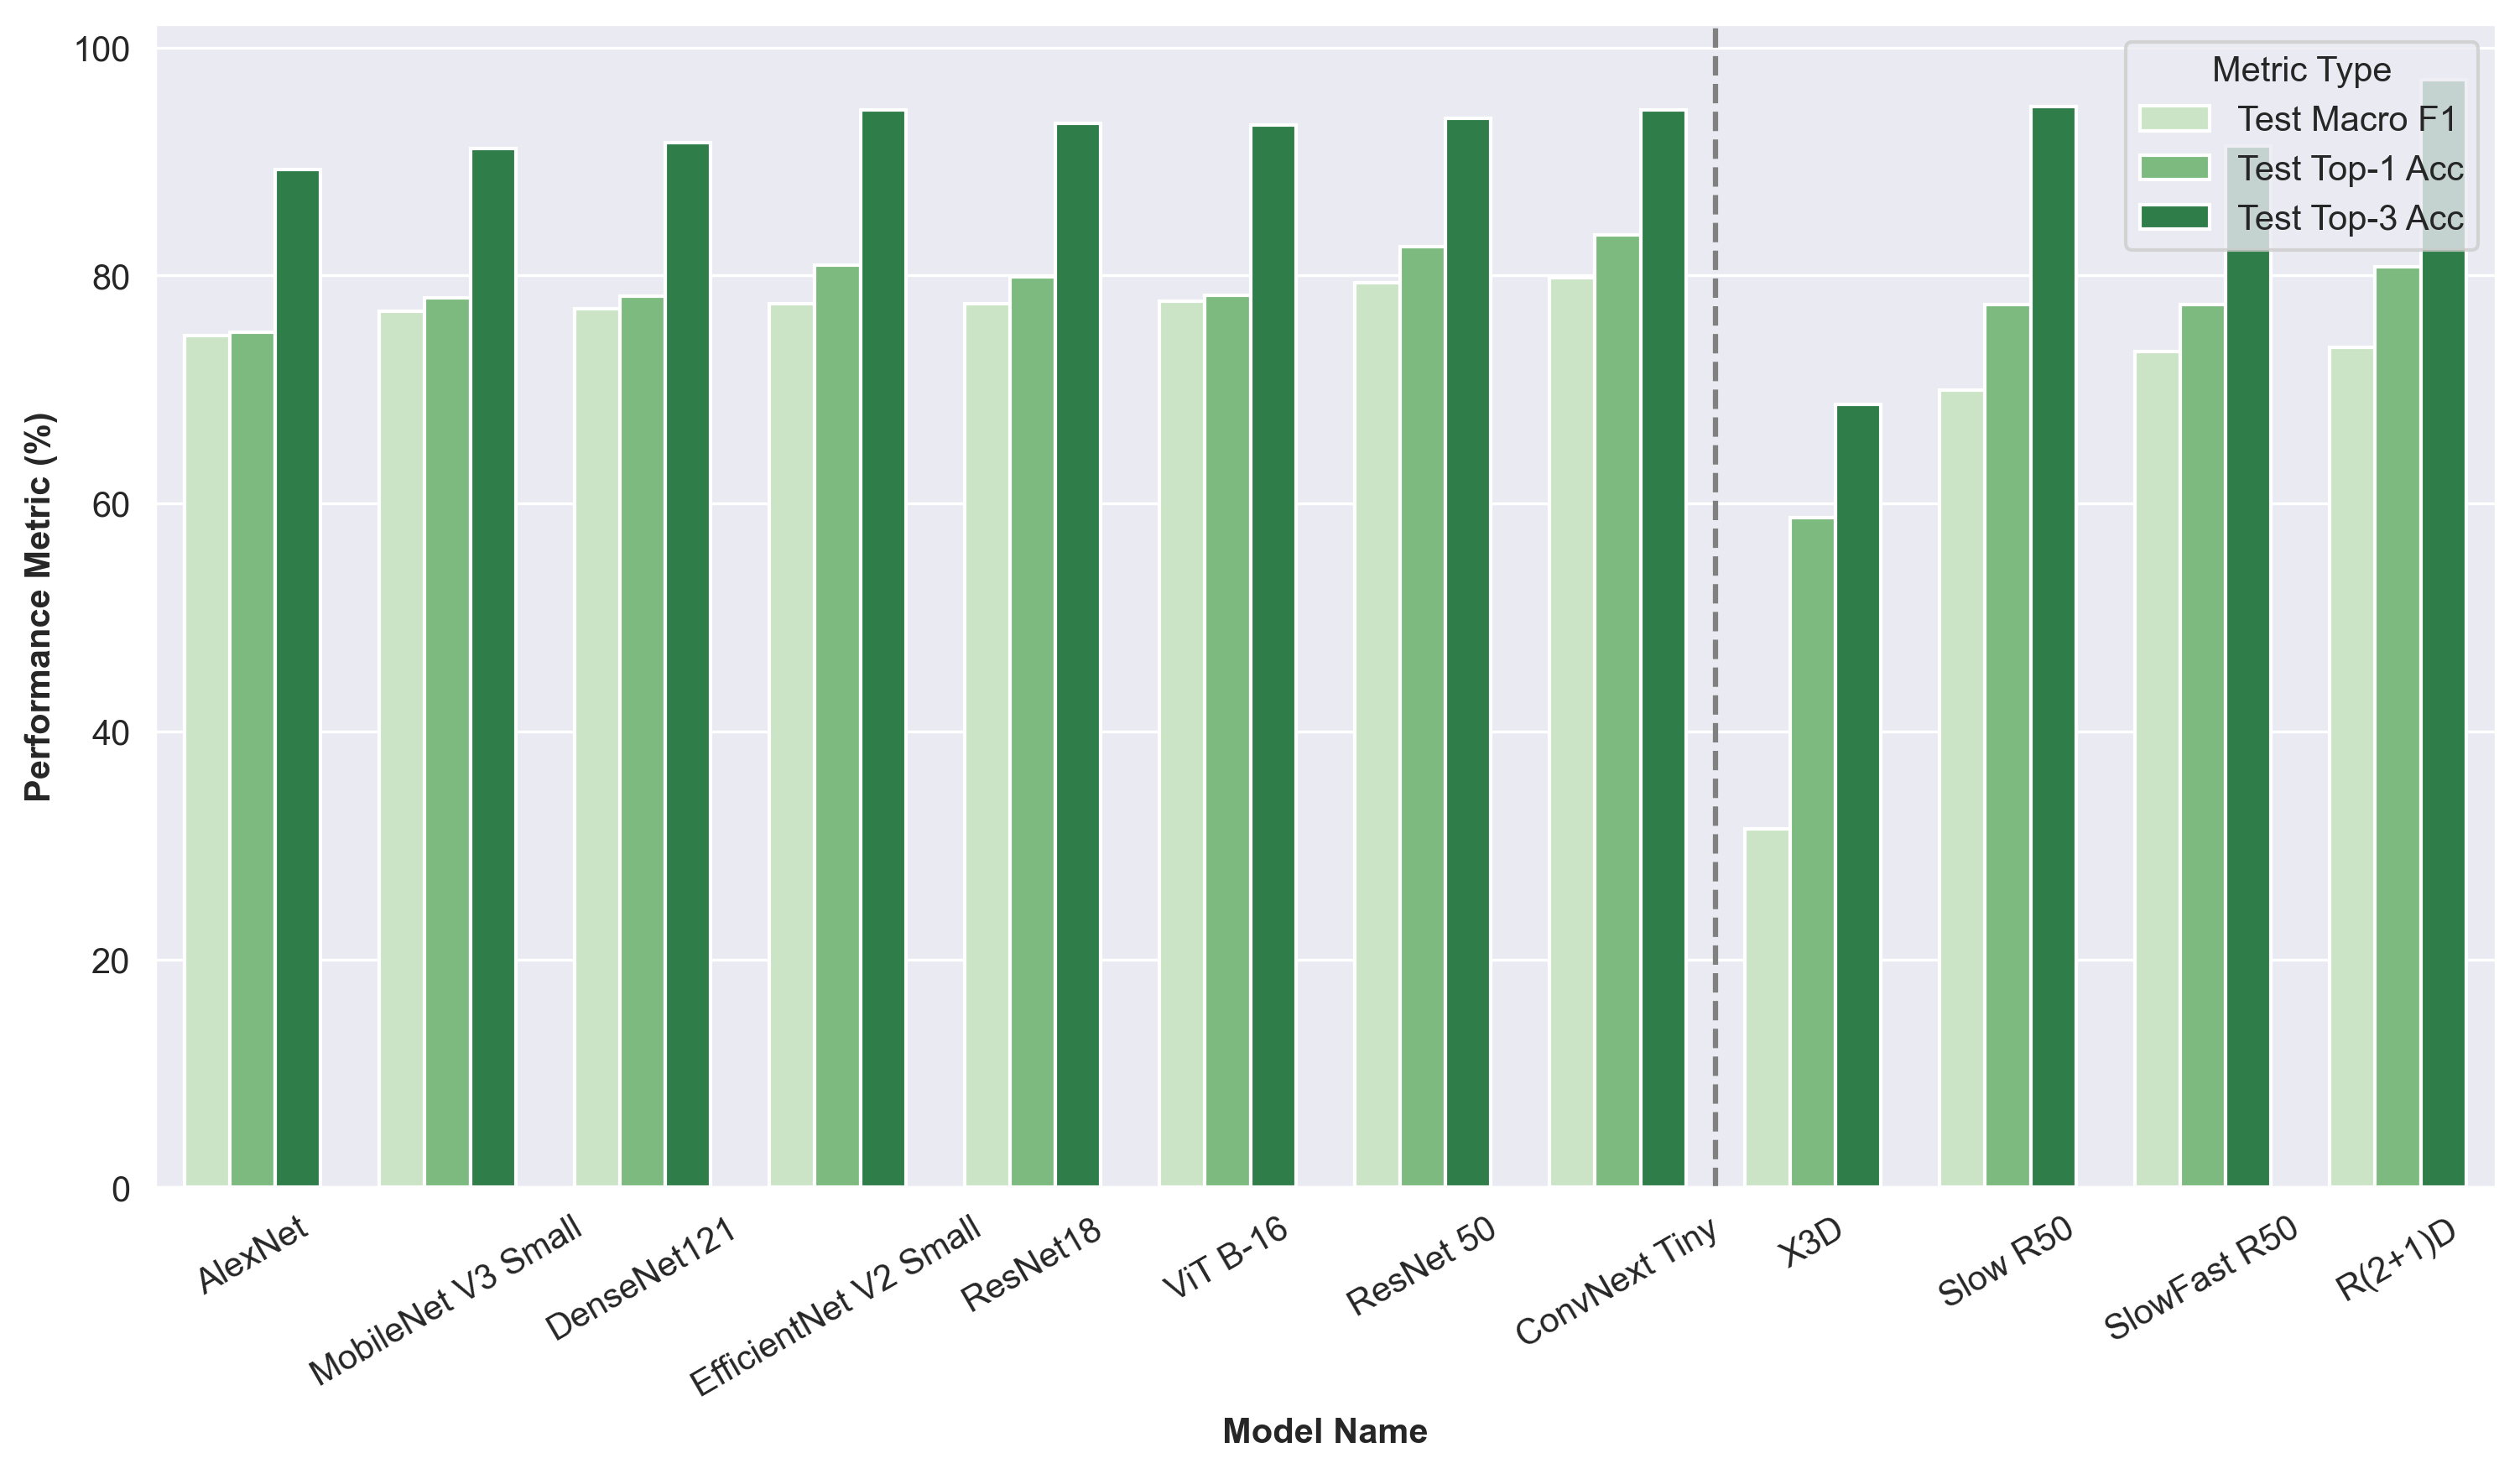
\includegraphics[width=.95\textwidth]
    {./figures/performance-metrics.png}
  \end{center}

  \caption{\textbf{Performance Metrics.} The Figure shows the performance
  metrics, Macro F1, Top-1 Accuracy and Top-3 Accuracy, for all trained models
on the test split. A grey, dotted line separates the single-frame classifiers
(left) from the video classifiers (right).}

  \label{fig:performance-metrics}
\end{figure}

\subsection{Efficiency Analysis} % (fold)
\label{sub:efficiency}

In deep learning, more complex models generally outperform simpler ones if
provided with sufficient training data and computing resources. However, there
is a trade-off between model complexity and efficiency, especially when
efficiency is critical, like when deployed on a mobile device.

The efficiency of the single-frame and video classifiers generally varies more
than the performance - within and between the groups of singe-frame and video
classifiers. The single-frame classifiers range from a throughput rate of 7.99
predictions per second (ViT-B-16) to 109.07 predictions per second (MobileNet V3
S). Three models (MobileNet V3 S, AlexNet, ResNet 18) can provide predictions in
real-time (at least 30 predictions per second). The video classifiers require
more computing and memory resources during inference and are less efficient.
They are only able to provide predictions between 1.26 predictions per second
(Slow R50 Family) and 3.01 predictions per second (R(2+1)D). However, as each
prediction considers a history of frames, the predictions are more robust and
valid for longer.

% tradeoff
Given these findings, it is clear that performance gains can be achieved with an
increased model complexity. However, small gains come at a high cost in terms of
efficiency. Figure~\ref{fig:tradeoff} visualises the performance-efficiency
trade-off for all models by plotting the relationship between the Top-1 Accuracy
against the latency (inference time in milliseconds per prediction) and the
throughput (predictions per second). Depending on the specific deployment
requirements, different models are more suitable. If low memory consumption and
high throughput are critical, high efficiency models like MobileNet V3 S are
most suitable. If the real-time inference is not critical but high accuracy is
required, models like ResNet50 or ConvNext Tiny are best suited. If more robust
but less frequent predictions are required, video classifiers like R(2+1)D can
be valid options.

\begin{figure}
\centering
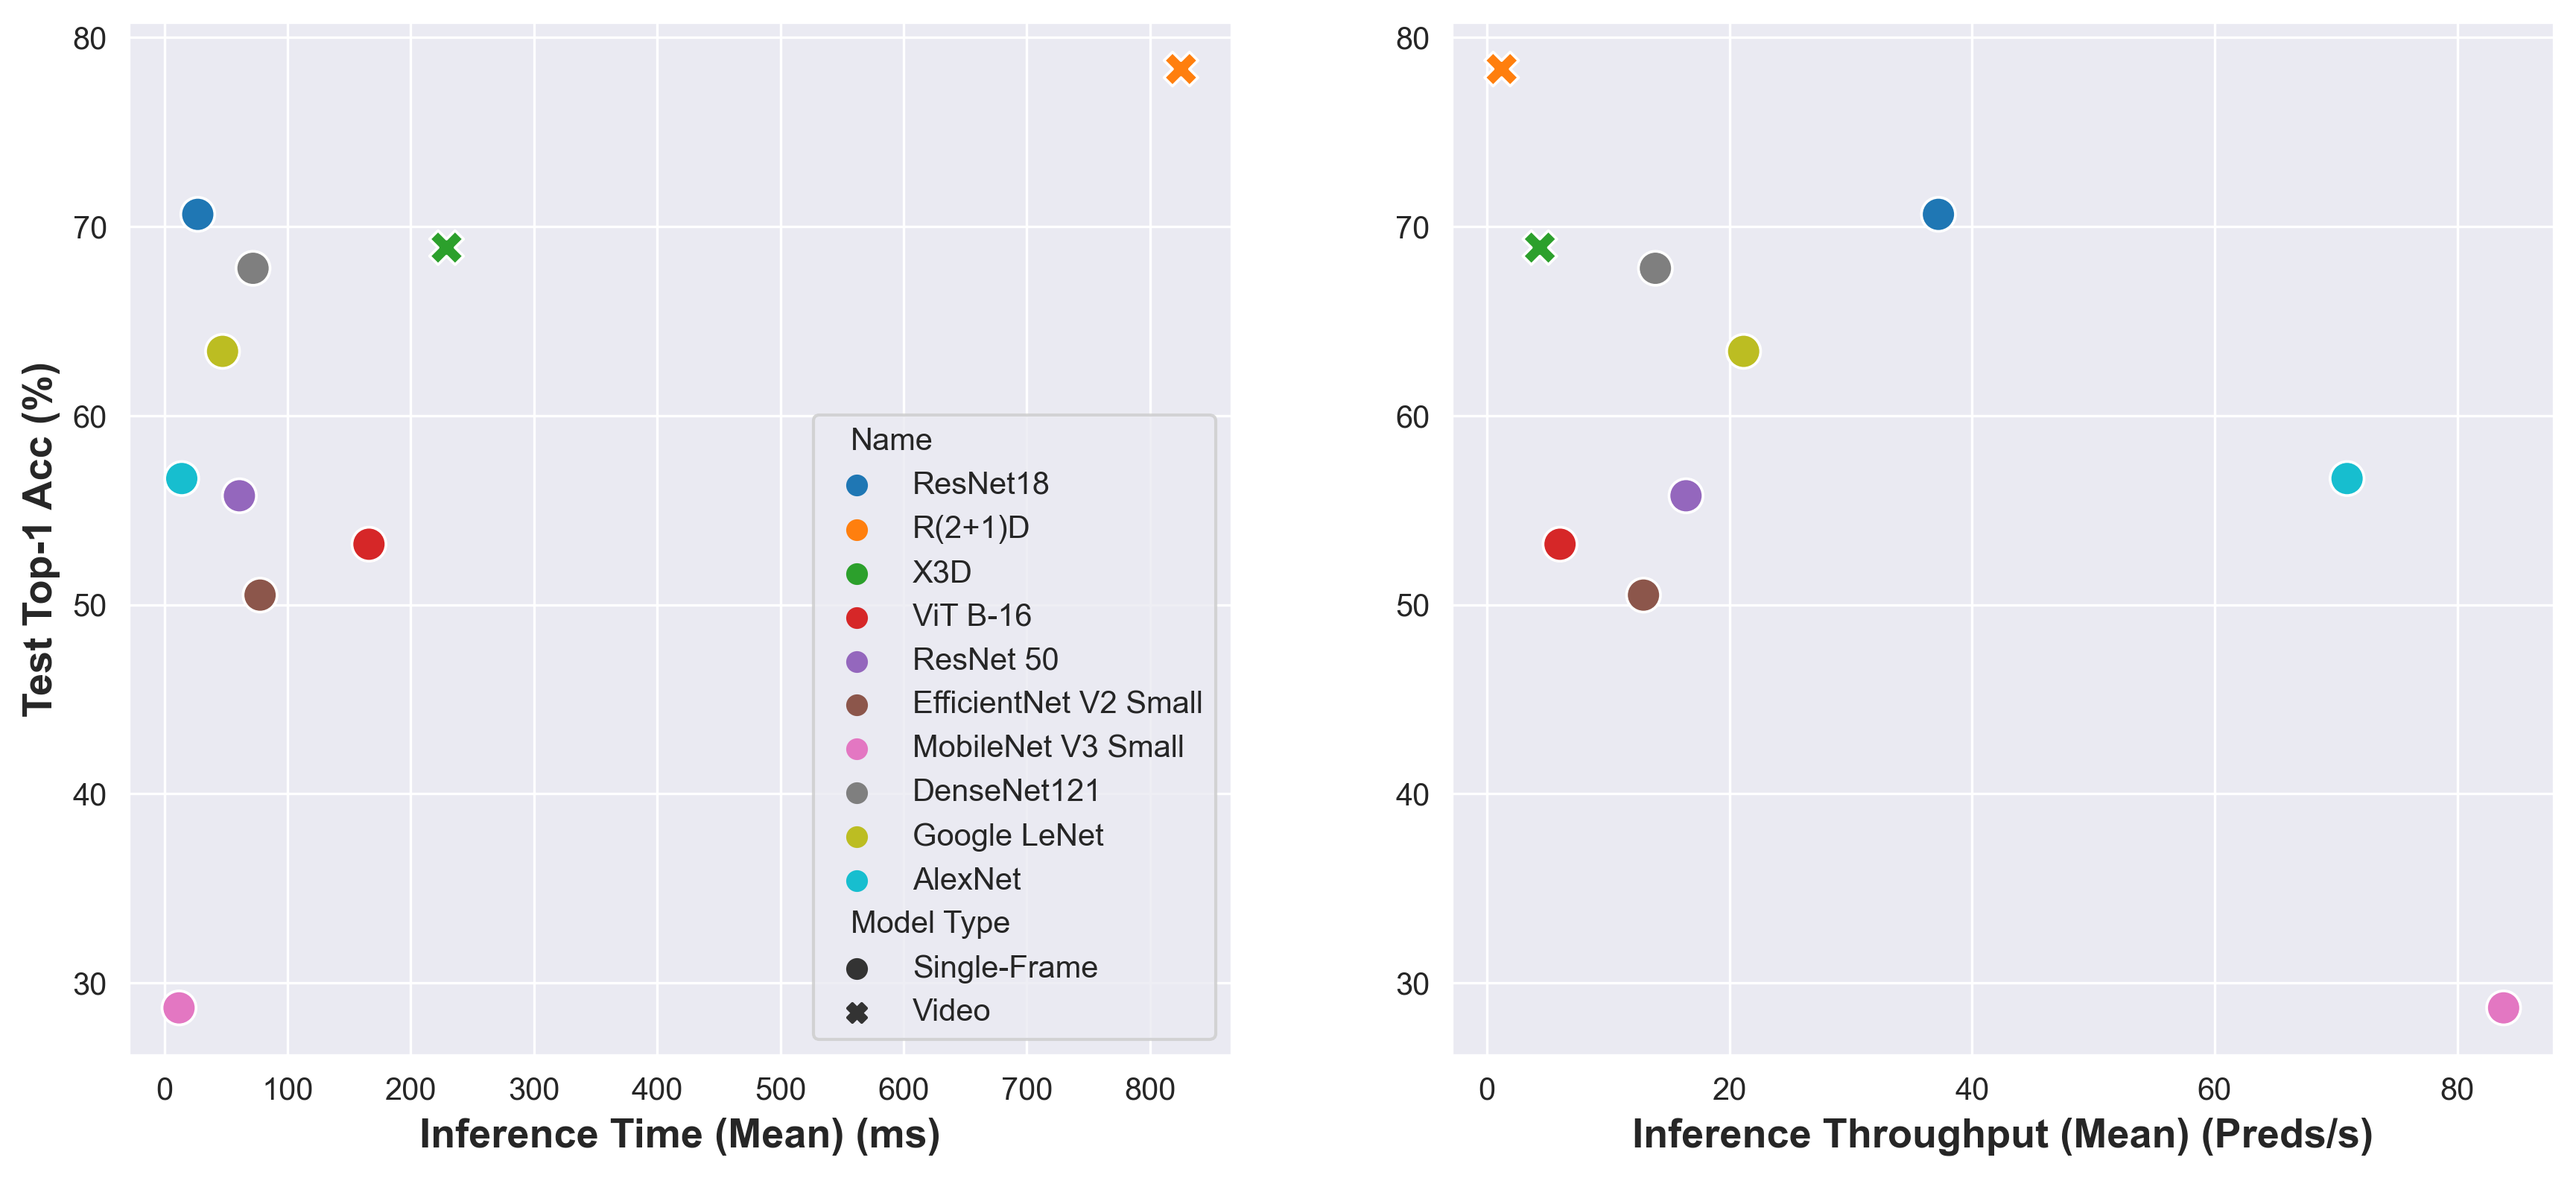
\includegraphics[width=\textwidth]{
./figures/performance-efficiency-tradeoff-scatter.png}
\caption{
  \textbf{Performance-Efficiency Trade-Off.} The Figure visualises the
  performance-efficiency trade-off for all models by plotting the
  relationship between the Top-1 Accuracy against the latency (inference
  time in milliseconds per prediction) and throughput (predictions per
  second). Each model is given unique colour, and the marker type indicates
  whether the model is a single-frame classifier (cross) or a video
  classifier (video).
}

\label{fig:tradeoff}
\end{figure}

% subsection tradeoff (end)

\subsection{Understanding Model Behaviour} % (fold)
\label{sub:conf-matrices}

To better understand the complex dynamics, strengths and weaknesses of deep
learning models in tackling the task of indoor classification, the two best
performing models in each group, ConvNext Tiny and R(2+1)D, are analysed in more
detail.

\subsubsection{Confusion Patterns} % (fold)

Figure~\ref{fig:conf-matrix} shows the confusion matrices for (a) ConvNext Tiny
and (b) R(2+1)D. Although the two models have very different
architectures, they exhibit similar confusion patterns.

\begin{figure}
  \centering
  \begin{subfigure}[b]{0.49\textwidth}
    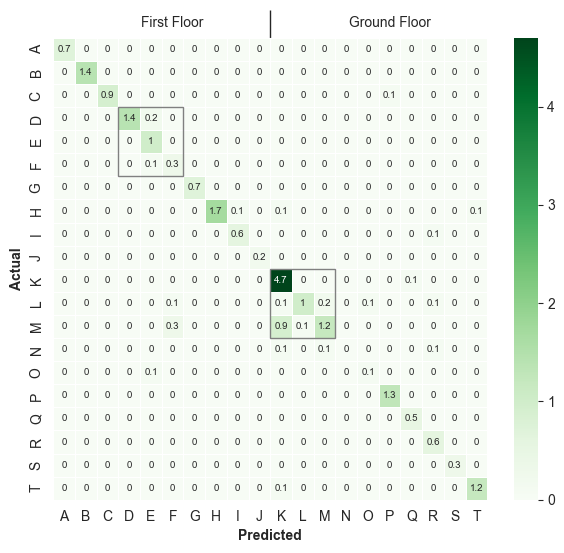
\includegraphics[width=\textwidth]{./figures/conf-matrix-convnext_tiny.png}
    \caption{ConvNext Tiny}
  \end{subfigure}
  \begin{subfigure}[b]{0.49\textwidth}
    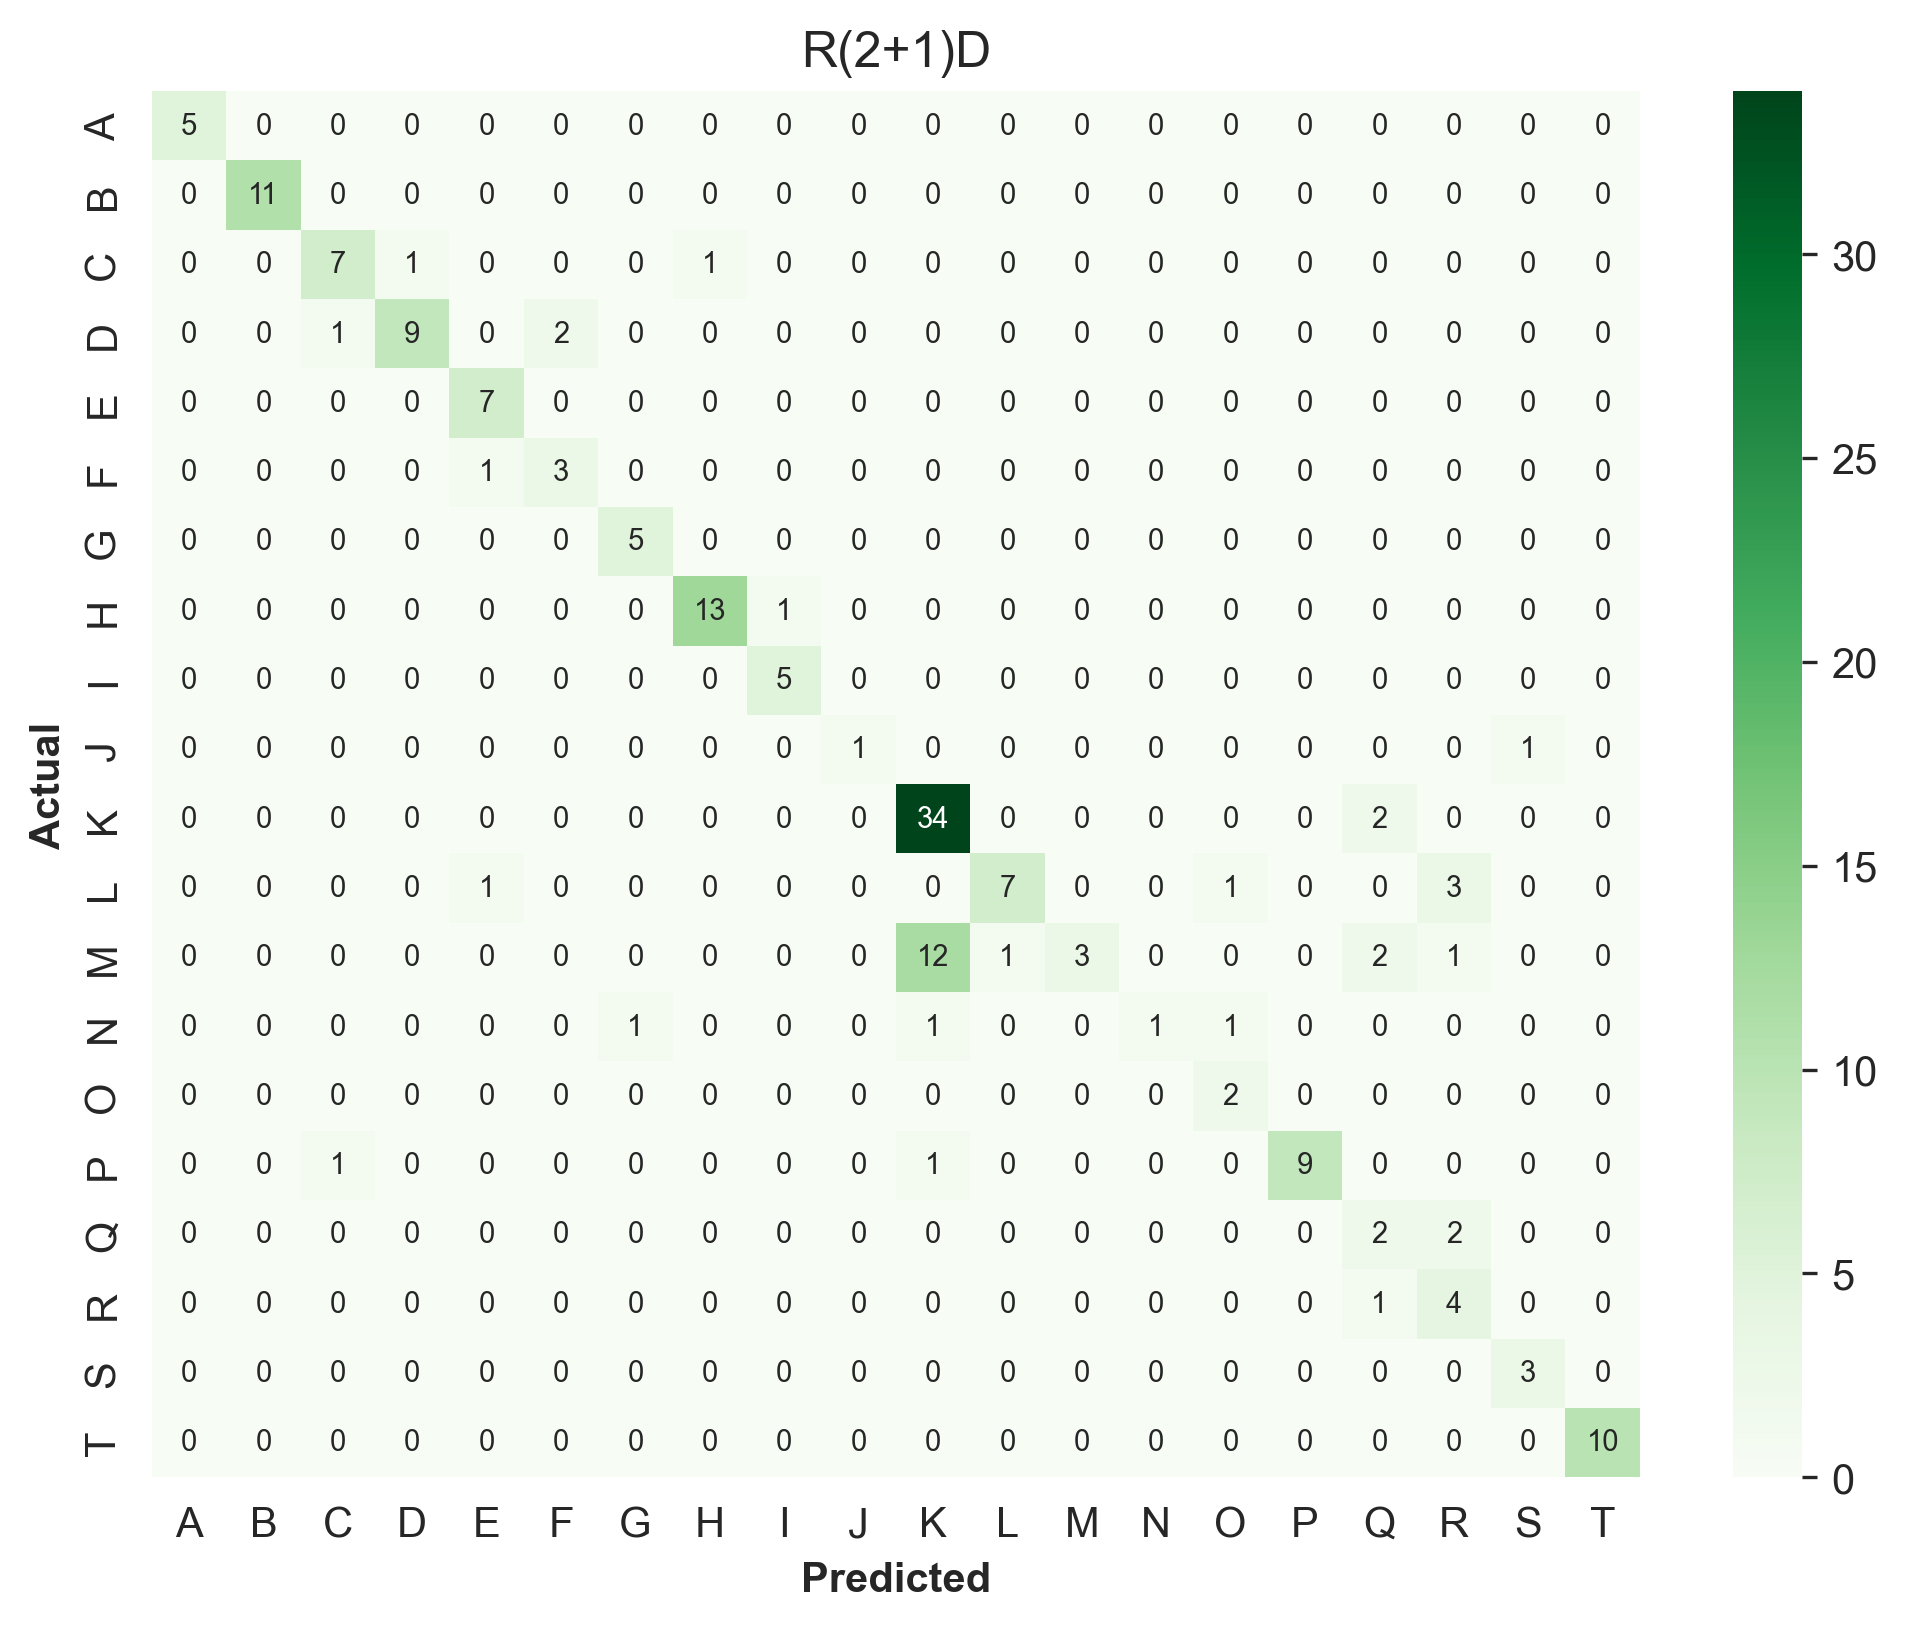
\includegraphics[width=\textwidth]{./figures/conf-matrix-r(2+1)d.png}
    \caption{R(2+1)D}
  \end{subfigure}
  \caption{ \textbf{Confusion Matrices.} The Figure shows the confusion matrix
    for (a) ConvNext Tiny and (b) R(2+1)D. The confusion matrix of ConvNext Tiny
    is normalised by a factor of 1/1000 for visual purposes. For both matrices,
    the entry at row $i$ and column $j$ shows the number of samples that belong
  to class $i$ but were predicted to be class $j$. Gray rectangles indicate
challenging subsets of classes, that are often confused. These are displayed in
more detail in Figure~\ref{fig:conf-matrix-challenging}. }
  \label{fig:conf-matrix}
\end{figure}

% confuses visually similar classes
Both models show a tendency to confuse visually similar classes. The first
example is the two corridors on the ground floor (Ground Floor Corridor 1 and
Ground Floor Corridor 2) and the atrium (Ground Floor Atrium). The corridor's
architecture, interior design and lighting are very similar, making it more
challenging for both models to distinguish between the two.
Figure~\ref{fig:conf-matrix-challenging}a shows the confusion between these
classes for both models in detail. ConvNext Tiny tends to predict the atrium
instead of the second corridor and regularly mixes up the two corridors. R(2+1)D
is less prone to confusing the two corridors but also mispredicts the second
corridor as the atrium in a few instances.

A second example is the three libraries (First Floor Library 1, First Floor
Library 2 and First Floor Library 2). The libraries are visually similar, as
they share similar characteristics, like bookshelves, tables and chairs.
Figure~\ref{fig:conf-matrix-challenging}b shows the confusion between these
classes for both models. ConvNext Tiny is more capable of differentiating the
three libraries but still confuses the first and second libraries. Weirdly,
R(2+1)D cannot differentiate between the libraries and predicts the second
library naively. This might be, because it is the most commonly occurring
library in the training data, and the model is therefore biased towards this
class.

% mispredicting majority class in cases of uncertainty
The above failure cases highlight another intricacy of the models: While
locations that are less present in the training data are generally handled well,
the models tend to predict the majority class in cases of uncertainty.

\begin{figure}
  \centering
  \begin{subfigure}[b]{\textwidth}
    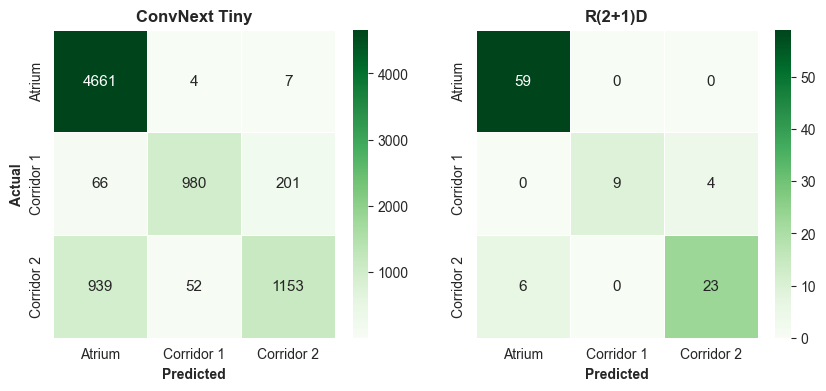
\includegraphics[width=\textwidth]{./figures/conf-matrix-corridors.png}
    \caption{Corridors}
  \end{subfigure}
  \vspace{.5cm}
  \begin{subfigure}[b]{\textwidth}
    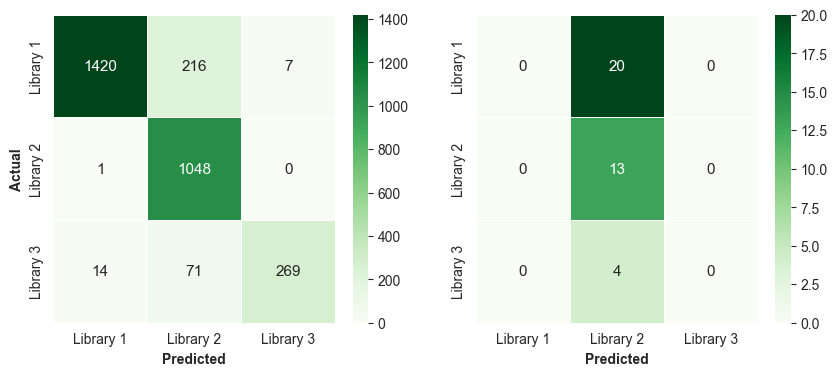
\includegraphics[width=\textwidth]{./figures/conf-matrix-libraries.png}
    \caption{Libraries}
  \end{subfigure}
  \caption{
    \textbf{Common Misprediction Patterns.} The figure shows subsets of the
    confusion matrices that highlight classes that are commonly confused by
    ConvNext Tiny (left) and R(2+1)D (right). Figure (a) shows the confusion
    between the two corridors on the ground floor and the Atrium. Figure (b)
    shows the confusion between the three libraries on the first floor. 
  }
  \label{fig:conf-matrix-challenging}
\end{figure}

\subsubsection{Misprediction Cases} % (fold)
\label{sub:mispredictons}

Exemplary mispredictions are analysed for both models confirm the above
findings. Figure~\ref{fig:mispredictions} displays six exemplary mispredictions
for ConvNext Tiny (Figure~\ref{fig:mispredictions}a) and R(2+1)D
(Figure~\ref{fig:mispredictions}b) each. The six mispredicted samples are
grouped into three commonly found misprediction patterns:

\textbf{Visual Similarities.} This pattern describes mispredictions between
visually similar classes. In the case of this study, there are several pairs or
triples of classes (e.g. the two corridors, three libraries), which share many
visual characteristics. The two samples in this group for ConvNext Tiny
uncover another of such groupings: the coloured areas on the ground and first
floor. The model is visibly less sure about the prediction, and the true class
is typically the second most confident prediction. For R(2+1)D, the first sample
shows confusion between the libraries, and the second sample shows confusion
between the two corridors on the ground floor.

\textbf{Location Transitions.} This pattern describes mispredictions between
classes that occur during the transition between areas. The first sample for
ConvNext Tiny is a clip that just passes the door between two libraries. The
model predicts the library before the door is passed, and the ground truth label
is the library after the door is passed. The second sample shows a similar case,
where the model predicts to be in the red area on the first floor, but the
ground truth label is still the class before. This confusion pattern naturally
arises because locations may not be sharply separable only from the imagery of a
camera. For example, if the camera only captures the features of the location
that lies a few meters ahead, it is likely that the model predicts the location
that lies ahead, but the ground truth label is still the location that lies
behind.

\textbf{Environment Change.} A third, interesting pattern was observed for both
models in the area that was renovated in between the data collection
periods for the training and testing split. Parts of Corridor 2 on the ground
floor were renovated and repainted in blue. Both models fail to recognise this
area and typically fall back to the two most common classes in the training
data, which is the Atrium and Library 2.

\begin{figure}
\centering

\begin{subfigure}[b]{\textwidth}
\centering
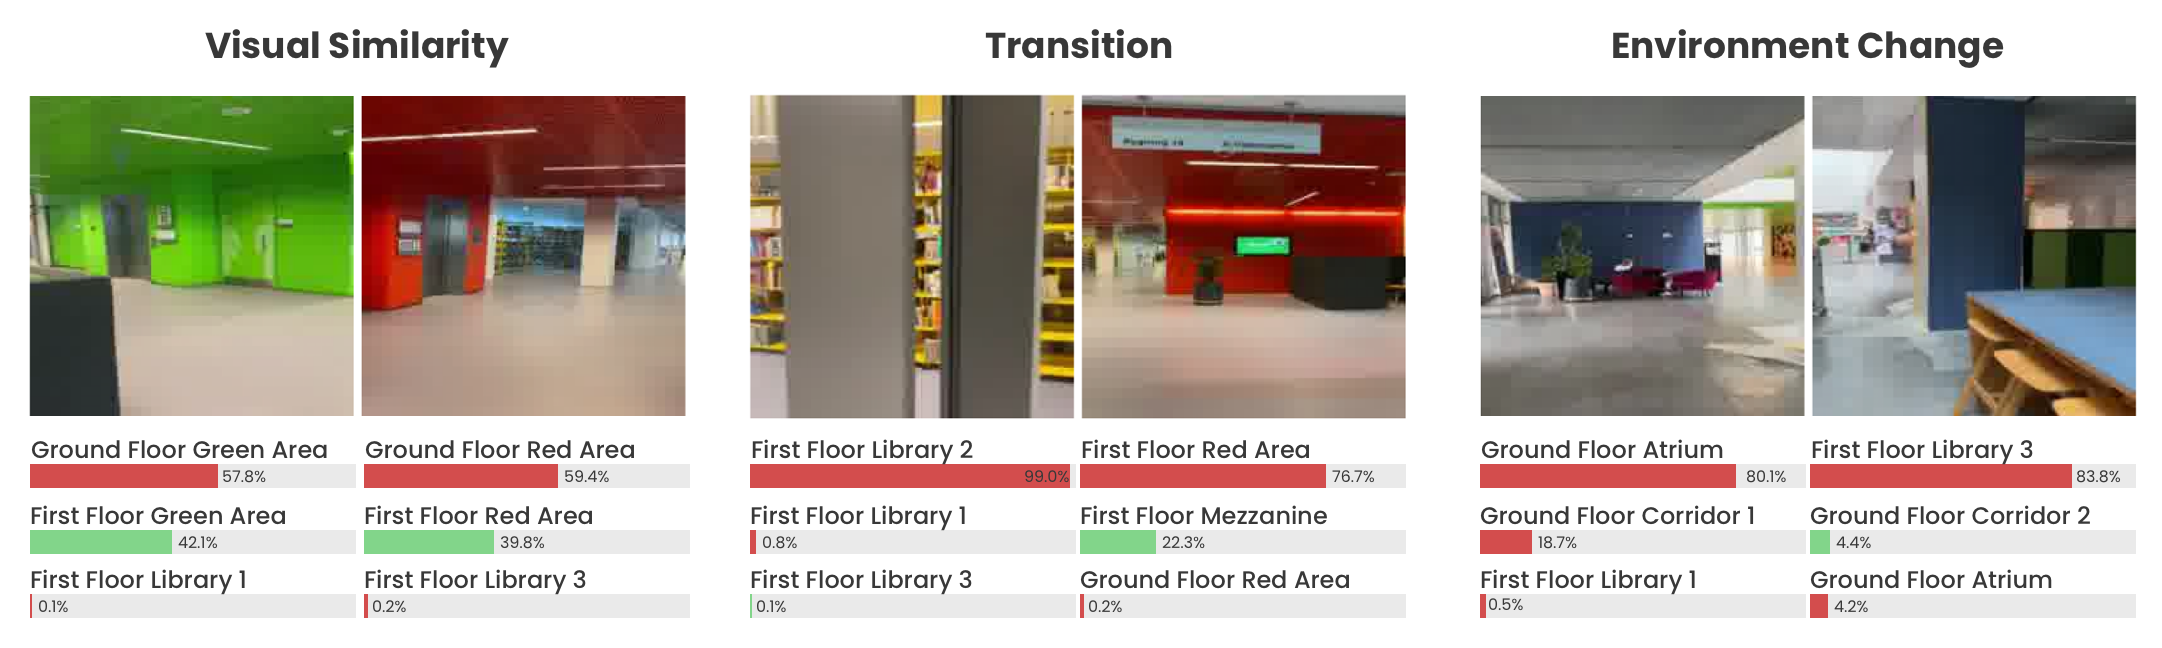
\includegraphics[width=\textwidth]{./figures/mispredictions-convext-tiny.png}
\caption{Misprediction Patterns for ConvNext Tiny}
\end{subfigure}

\begin{subfigure}[b]{\textwidth}
\centering
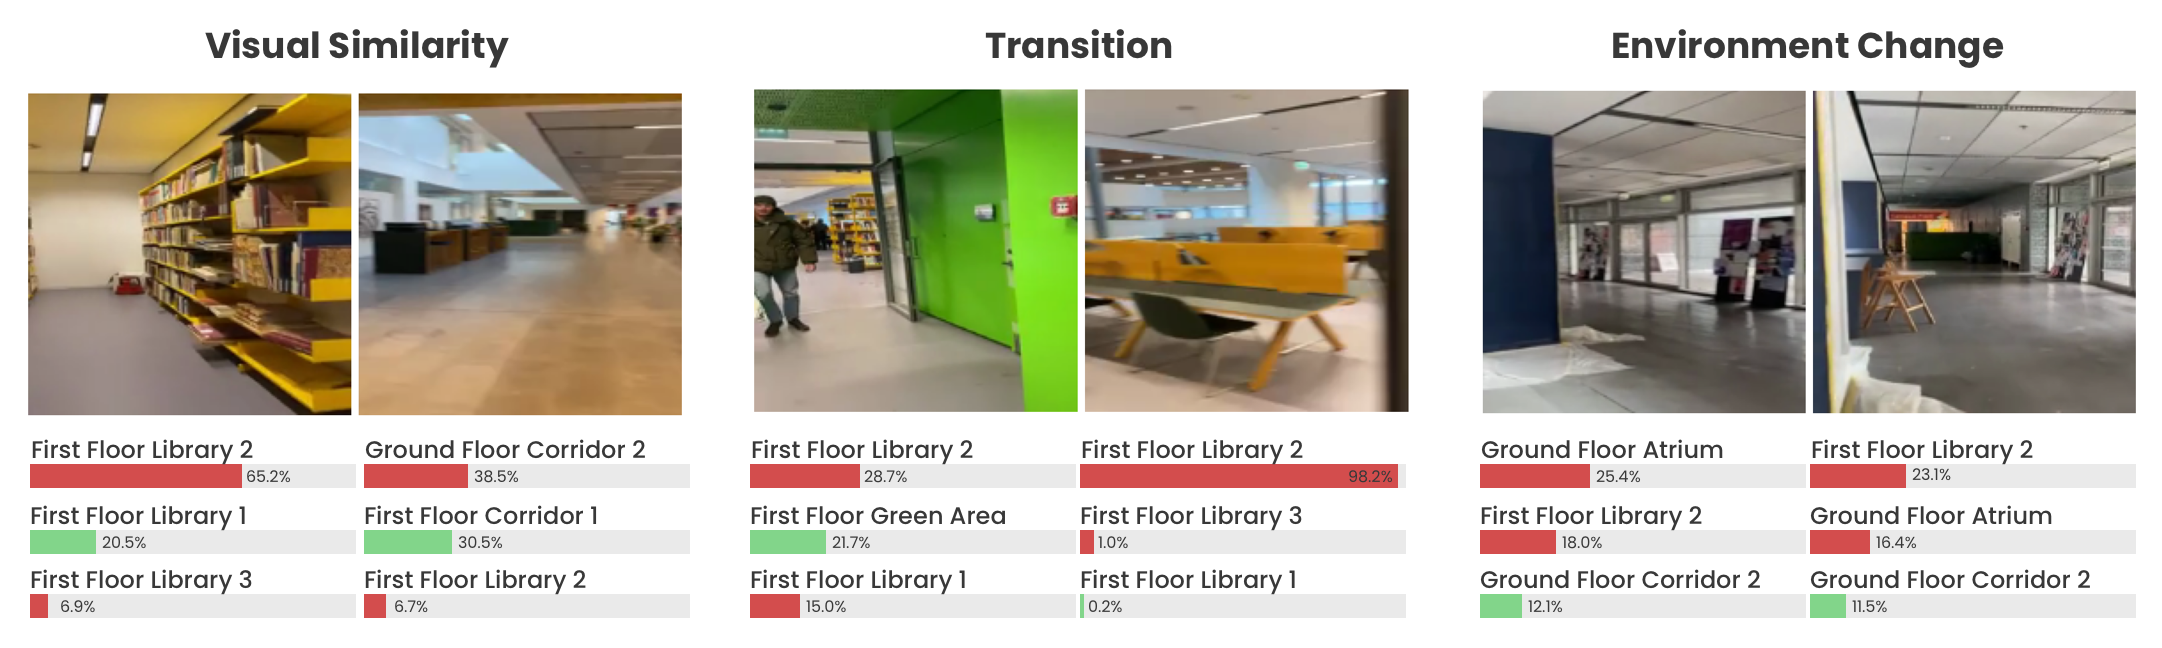
\includegraphics[width=\textwidth]{./figures/mispredictions-r2plus1d.png}
\caption{Misprediction Patterns R(2+1)D}
\end{subfigure}

\caption{\textbf{Mispredicted Samples.} Exemplary mispredicted samples for (a)
  ConvNext Tiny and (b) R(2+1)D. For each sample, the top 3 predicted classes
  are shown in order of confidence. The true class, if among the top 3
  predictions, is highlighted through a green bar. The mispredicted samples are
  grouped in the three commonly observed misprediction patterns: (1) Visual
  Similarity (2) Transition and (3) Environment Change. For the clips from the
  video classifier, the first frame of the clip is shown.}
\label{fig:mispredictions}
\end{figure}

% subsection mispredicted (end)

\subsubsection{Model Behaviour Analysis} % (fold)
\label{sub:behaviour}

Finally, to emulate the behaviour of the models in a real-world scenario, both
ConvNext Tiny and R(2+1)D continuously predicted the location in all videos in
the test split. As a result, the following additional qualitative observations
were made:

\textbf{Prediction Consistency.} The single-frame classifier, ConvNext Tiny, was
more inconsistent in its predictions than the video classifier, R(2+1)D. In
complex cases, like the ones described in the previous section, ConvNext Tiny
would often predict different classes in a short time span, leading to "flicker"
in the predictions. This behaviour was almost absent in R(2+1)D due to
the lower throughput rate and its temporal modelling capabilities, which allow
the model to smooth out predictions over time.

\textbf{Training Data Bias.} A bias toward the training data is present in both
models. If features are not representative of a location but are overrepresented
in the training data of that location, there is a chance for the model to learn
these features as indicative of a class. This was the case for the libraries:
Most video clips that were taken while walking through bookshelves were filmed
in library 2, while the other libraries were filmed in a more open space. This
led to models associating in-between bookshelves clips to library 2, even though
they are also present in the other libraries.

% subsection manual (end)

\subsection{Deployment on Mobile Devices}
\label{sub:deploment}

As a proof of concept, the most efficient and mobile-optimised model, MobileNet
V3 Small, was deployed on a mobile device. The trained model was quantised to
8-bit float precision, converted to the \texttt{TorchScript} format, and finally
deployed using the \texttt{PlayTorch} framework. The deployed model can be
tested by downloading the PlayTorch app from the App Store or Google Play Store
and scanning the QR code found in the
\href{https://github.com/mikasenghaas/bsc}{README} of this project's GitHub
repository. After scanning the QR code within the PlayTorch app, the model will
be downloaded and run locally on the device.

% subsection deployment (end)

% section results (end)
\section{Conclusion}

\subsection{Limitations \& Future Work} % (fold)
\label{sub:limitations}

% This study has shown the potential of using common deep learning methods for
% providing accurate room-level localisation. 

% small dataset
Arguably, the most significant limitation of this study is the small dataset
used for training and evaluation. 

% small training set
The problem is two-fold: First, the relatively small training set leads to the
models only seeing a subset of the possible angles, routes and natural
variations in indoor spaces. As a result, consequences were visible in the
misprediction patterns, as models often confused visually similar locations.
Second, the small evaluation set might not represent the variation of visual
inputs from an indoor location over a year. Therefore, this study's evaluation
might not capture the potential weaknesses of the models in real-world
deployment.

% for this reason, investigate how the models perform on a larger dataset and in
% more complex environments
Therefore, a sensible next step would be to collect a larger dataset that
captures the full variation of visual inputs from an indoor location over a long
period of time. This would allow to investigate if more training data can
overcome some of the misprediction patterns observed in this study. An
interesting follow-up research question that speaks to the practicality of the
proposed methodology is \textit{how much} data is needed to achieve a certain
level of accuracy; ideally, as little data as possible should be collected to
reduce data collection and annotation cost while maintaining a high level of
accuracy.

% regarding mispredictions patterns: 1. visual similarity 2. transition 3.
% environment change, three can't be changed, 2. is difficult, but also not that
% bad in real-wordl deployment and 1. is either solved by more data or by
% directly incorporating relative location information

% misprediction patterns
Finally, the detailed analysis of the mispredicted samples has revealed three
frequent misprediction patterns: The fact that models depending on the modality
of vision alone are unable to maintain high accuracy when drastic changes in the
environment occur is a fundamental limitation of the proposed methodology, and
likely cannot be overcome without major changes to the methodology. The second
pattern, mispredictions at transitions between rooms, is also inherent to the
task of room-level localisation, as it is sometimes hard to clearly distinguish
when a transition occurs. Future work could investigate how to make transitions
more smooth. Lastly, the confusion of visually similar classes is the problem
that is most likely to be solvable. As mentioned, the first step would be to
collect more data to allow the models to learn more discriminative features.
Another starting point might be to directly incorporate the relative position of
the rooms in the building, which could limit the number of possible predictions.
For example, if a model is confident in predicting the current room, it could
use this information to limit the number of possible predictions for the next
frame if it has information about the current adjacent rooms.

\subsection{Summary} % (fold)
\label{sub:summary}

% indoor localisation is solvable with a pure deep learning pipeline
This study has demonstrated that it is possible to train deep learning models
and deploy them on mobile devices to provide reasonably accurate location
estimates in indoor spaces.

% performance
Both single-frame classifiers that only use static frames as input and video
classifiers that directly model the temporal information in videos, were capable
of learning discriminative features from the visual input that allows them to
localise a human agent in an indoor space from a set of rooms with a test
accuracy of up to 83.59\%. While the overall performance of models, also across
groups, was similar, video classifiers were more consistent and robust in their
predictions. However, this added robustness comes at the cost of a lower
throughput rate, making the models less suitable for deployment on mobile
devices.

% failure modes
A detailed analysis of the model's misprediction patterns and complex behaviours
of unveiled three frequent failure modes: The models struggled with visually
similar locations, transitions between locations and when significant visual
changes, such as renovations, occur in the environment. Furthermore, both models
were susceptible to biases in the training data, for example, if a feature that
is not representative of a location is overrepresented in the training data of
that location.

% promising results and outlook
Overall, the results are promising and suggest that with a larger-scale and
carefully designed dataset, it is possible to train models that can overcome the
limitations observed in this study to provide even more accurate location
estimates in indoor spaces. This could make the proposed method a viable
alternative to existing indoor localisation systems, for example, in indoor
navigation or augmented reality applications.

% bibliography
\newpage
\bibliography{references}
\bibliographystyle{abbrv}

\newpage
\section{Appendix} % (fold)
\label{sec:appendix}

\subsection{Reproducibility} % (fold)
\label{sub:reproducibility}

All code and data used in this project is available on
\href{https://github.com/mikasenghaas/bsc}{GitHub}. The project's
\texttt{README} file contains detailed instructions on how to reproduce the
results of this project.

Further, the precise configuration and results of the experiments that are
reported here are publicly available as a public
\href{https://wandb.ai/mikasenghaas/bsc}{Weights \& Biases} experiments.

% subsection reproducibility (end)

\subsection{Machine Specifications} % (fold)
\label{sub:machine-specs}

Table~\ref{tab:machine-specs} lists the two machines, alongside relevant
specifications, that were used for training and evaluation of the models.
The HPC cluster was used for training and evaluation of all models. Analyses
and visualisations were performed on the local machine, as well as running the
real-time inference demo. 

\begin{table}[ht]
  \centering
  \begin{tabular}{cll}

  \toprule
  & Specification & Value \\
  \midrule

  \multirow{2}{*}{\rotatebox[origin=c]{90}{Sys.}} 
  & Name & Linux \\
  \vspace{0.1cm}
  & Node & Desktop 24 \\

  \multirow{4}{*}{\rotatebox[origin=c]{90}{CPU}}
  & Model & Intel(R) Xeon(R) CPU E5-2660 v3 @ 2.60GHz \\
  & Architecture & x86\_64 \\
  & Physical Cores & 20 \\
  \vspace{0.1cm}
  & Frequency & 3.3 GHz \\

  \multirow{2}{*}{\rotatebox[origin=c]{90}{GPU}} 
  & Model & NVIDIA GeForce GTX 1080 Ti \\
  \vspace{0.1cm}
  & Memory & 11.2 GB \\

  \multirow{2}{*}{\rotatebox[origin=c]{90}{Mem.}}
  & Total Capacity & 250  
  GB\\
  & Avg. Used Capacity & $\sim 7.4$ GB \\

  \bottomrule
  \end{tabular}
\caption{\textbf{Machine Specifications.} The Table shows relevant hardware
specifications for the remote server that was used for conducting experiments
within this study.}

\label{tab:machine-specs}
\end{table}

% section remarks (end)

\end{document}
